\documentclass[oneside]{article}

\usepackage{blindtext} % dummy text
\usepackage{graphicx} % for figures
\usepackage{color} % for colored text
\usepackage{colortbl} % for colored text
\usepackage{float} % for forcing figure placement
\usepackage[breakable]{tcolorbox} % for text box
\usepackage{enumerate} % for bullet point lists
\usepackage{setspace} % line spacing
\usepackage{soul} % strike through
\usepackage[normalem]{ulem} % strike through keeping emphasis standard
\usepackage{cancel} % diagonal strike through
\usepackage[margin=1in]{geometry} % margins
\usepackage{lineno} % page numbers
\usepackage[sc]{mathpazo} % Use the Palatino font
\usepackage[T1]{fontenc} % Use 8-bit encoding that has 256 glyphs
% \linespread{1.05} % Line spacing - Palatino needs more space between lines
\usepackage{microtype} % Slightly tweak font spacing for aestheticsgins
\usepackage[small,labelfont=bf,up,up]{caption} % Custom captions under/above floats in tables or figures
\usepackage{booktabs} % Horizontal rules in tables
\usepackage{amsmath} % Text in equations
\usepackage{titlesec} % Allows customization of titles
\usepackage{titling} % Customizing the title section
\usepackage{listings} % listings environment
\usepackage[framemethod=TikZ]{mdframed} % nice listing frame
\usepackage[hidelinks]{hyperref} % For hyperlinks in the PDF

\usepackage{algorithm2e}

\usepackage{tikz}
\usetikzlibrary{shapes.geometric, arrows, positioning, decorations.markings, shapes.multipart}   
\usepackage{standalone}

\usepackage{subcaption} % for subfigures side by side
\captionsetup[subfigure]{singlelinecheck=false} % to put (a) and (b) at the top-left of subfigures

\usepackage[shortlabels]{enumitem} % customized lists (shortlabels
                                % necessary to have i., ii., etc., in enumerate)
\setlist[itemize]{noitemsep} % Make itemize lists more compact

\usepackage{abstract} % Allows abstract customization
\renewcommand{\abstractnamefont}{\normalfont\bfseries} % Set the "Abstract" text to bold
\renewcommand{\abstracttextfont}{\normalfont\small\itshape} % Set the abstract itself to small italic text

\usepackage{fancyhdr} % Headers and footers
\pagestyle{fancy} % All pages have headers and footers
\fancyhead{} % Blank out the default header
\fancyfoot{} % Blank out the default footer
\fancyhead[C]{Mendes et al. $\bullet$ December 2023 $\bullet$ bio{\color{red}R}$\chi$ve} % Custom header text
\fancyfoot[RO,LE]{\thepage} % Custom footer text

\usepackage{natbib}
\bibliographystyle{apalike}

\usepackage{libertine}

\lstdefinelanguage{XML}
{
  basicstyle=\ttfamily,
  morestring=[s]{"}{"},
  morecomment=[s]{?}{?},
  morecomment=[s]{!--}{--},
  commentstyle=\color{blue5},
  moredelim=[s][\color{black}]{>}{<},
  moredelim=[s][\color{pink2}]{\ }{=},
  stringstyle=\color{black},
  identifierstyle=\color{orange1}
}
\definecolor{light-gray}{gray}{0.95}
\definecolor{pink2}{RGB}{236,74,138}
\definecolor{orange1}{RGB}{255,102,0}
\definecolor{blue5}{RGB}{46,62,79}

\setlength\columnsep{20pt}

%----------------------------------------------------------------------------------------
%	TITLE SECTION
%----------------------------------------------------------------------------------------

\setlength{\droptitle}{-4\baselineskip} % Move the title up

%\pretitle{\begin{center}\Huge\bfseries} % Article title formatting
%\posttitle{\end{center}} % Article title closing formatting

\title{How to validate a Bayesian evolutionary model} % Article title
%LM: strictly speaking, we're 'validating' the inference machinery.
%% Validating a model involves epistemic considerations that are, as far as I understand, outside the scope of this paper.
\author{\textsc{F\'{a}bio K. Mendes$^{1\dagger*}$}, \textsc{Remco Bouckaert$^{2\dagger}$},\\
\textsc{Luiz M. Carvalho$^{3\dagger}$}, \textsc{Alexei J. Drummond$^{4}$} \\
\small $^1$Department of Biological Sciences, Louisiana State University, Baton Rouge, LA 70803, United States\\
\small $^2$School of Computer Science, The University of Auckland, Auckland 1010, New Zealand\\
\small $^3$Escola de Matem\'{a}tica Aplicada, Fundaç\~{a}o Getulio Vargas, Rio de Janeiro, RJ 22250-900, Brazil\\
\small $^4$School of Biological Sciences, The University of Auckland, Auckland 1010, New Zealand\\
\small
\href{mailto:fmendes@lsu.edu}{$^*$Corresponding author: fmendes@lsu.edu}\\
{\small $^\dagger$Authors contributed equally to this work}
%\and % Uncomment if 2 authors are required, duplicate these 4 lines if more
%\textsc{Jane Smith}\thanks{Corresponding author} \\[1ex] % Second author's name
%\normalsize University of Utah \\ % Second author's institution
%\normalsize \href{mailto:jane@smith.com}{jane@smith.com} % Second author's email address
}
\date{\today} % Leave empty to omit a date

\renewcommand{\figurename}{Supplementary Figure}
\renewcommand{\tablename}{Supplementary Table}

\doublespacing

\linenumbers


% \usepackage{listings}
\begin{document}

\maketitle

\begin{center}
    \Large Supplementary Material
\end{center}

\newpage


% \section{Additional validation examples and guidelines}

\section{Examples of software for evolutionary model simulation}

\begin{center}
  \begin{table}[h]
  \caption{A non-exhaustive list of simulation software used for various models in evolutionary biology.}
  \label{suptab:sim}
  \centering
  \begin{tabular}{ p{0.7in} p{1.5in} p{1in} p{1.3in} }
    \hline
    Software package & Model type & Platform & Reference \\
    \hline  
    \rowcolor{gray!10}Seq-Gen & Molecular sequence evolution models & Standalone & \citealp{rambaut97} \\
    ms & Coalescent model & Standalone & \citealp{hudson02}\\
    \rowcolor{gray!10}msprime & Coalescent model & Python & \citealp{kelleher16}\\
    SLiM & Population genetic models & Standalone & \citealp{haller19}\\    
    \rowcolor{gray!10}mvMORPH & Continuous trait evolution models & R & \citealp{clavel15}\\
    TreeSim & Birth-death models & R & \citealp{stadler11}\\
    \rowcolor{gray!10}diversitree & Several birth-death models & R & \citealp{fitzjohn12}\\
    castor & Several birth-death models & R & \citealp{castor}\\
    \rowcolor{gray!10}PhyloJunction & Several birth-death models & Python & \citealp{mendes24}\\
    ReMASTER & Several birth-death models & BEAST 2 & \citealp{vaughan24}\\
    \rowcolor{gray!10}RPANDA & Several evolutionary models & R & \citealp{rpanda}\\
    LPhy & Several evolutionary models & Standalone & \citealp{drummond23}\\
    \rowcolor{gray!10}RevBayes & Several evolutionary models & RevBayes & \citealp{revbayes}\\
    \hline
  \end{tabular}
  \end{table}
\end{center}

\section{Validating a phylogenetic Brownian motion simulator}

One commonly used model in macroevolution for the study of continuous traits is the phylogenetic Brownian motion model (``PhyloBM'' in Fig. 1 of the main text; \citealt{fel73}).
The pdf characterizing this model's sampling distribution is in fact the pdf of the multivariate normal (MVN) probability distribution:

\begin{equation}
  \begin{split}
    \text{log }f(\boldsymbol{y} \mid \boldsymbol{y_0}, r, \boldsymbol{T}) = -\frac{1}{2} \Big[ n\text{log}(2\pi) + \text{log}|r \boldsymbol{T}| \Big] & \\
    -\frac{1}{2} \Big[ (\mathbf{y} - \boldsymbol{y_0})^T (r \boldsymbol{T})^{-1} (\mathbf{y} - \boldsymbol{y_0}) \Big].
  \label{eq:bm}
  \end{split}
\end{equation}

\noindent This probability density function describes the distribution obtained from an infinite number of BM ``experiments'' (each experiment being non-mean-reverting, and representing an independent evolutionary trajectory).
Under this model, one has data $d = \{\boldsymbol{y}\}$ and parameters $\boldsymbol{\theta} = \{\boldsymbol{y_0}, r, \boldsymbol{T}\}$ (sometimes researchers treat $\phi$ and consequently $\boldsymbol{T}$ as data instead of as a parameter).

The data, $\boldsymbol{y}$, corresponds to the observed values of a trait scored for $n$ species.
Among the parameters, $\boldsymbol{y_0}$ is the trait value at the root of the tree, $r$ is the instantaneous rate of change (i.e., the evolutionary rate, and sometimes represented by $\sigma^2$), and $\boldsymbol{T}$ is a matrix whose elements are deterministically defined by tree $\phi$'s topology and branch lengths.
Matrix $r\boldsymbol{T}$ is also known as the variance-covariance matrix; as an example, such matrix in supplementary figure \ref{fig:bmsim} would evaluate to:

\begin{equation}
  r\boldsymbol{T} = 0.1
  \begin{bmatrix}
    6 & 5 & 0\\
    5 & 6 & 0\\
    0 & 0 & 6
  \end{bmatrix}
  \label{eq:mat}
\end{equation}

\noindent Together with $\boldsymbol{y_0} = [0.0, 0.0, 0.0]$, this matrix characterizes a population of phylogenetically related species trait values whose means are 0.0, variances are 6.0, and co-variances are 5.0 (between species ``A'' and ``B'') and 0.0 (between species ``C''and either ``A'' or ``B'').
Supplementary figure \ref{fig:bmsim} shows the distributions of trait values and their variances and covariances for one sample of one thousand independent realizations of phylogenetic BM processes. 
One can see that the sample's average trait value and the variances and covariances approach their expectations. 

\begin{figure}[h!]
  \centering
  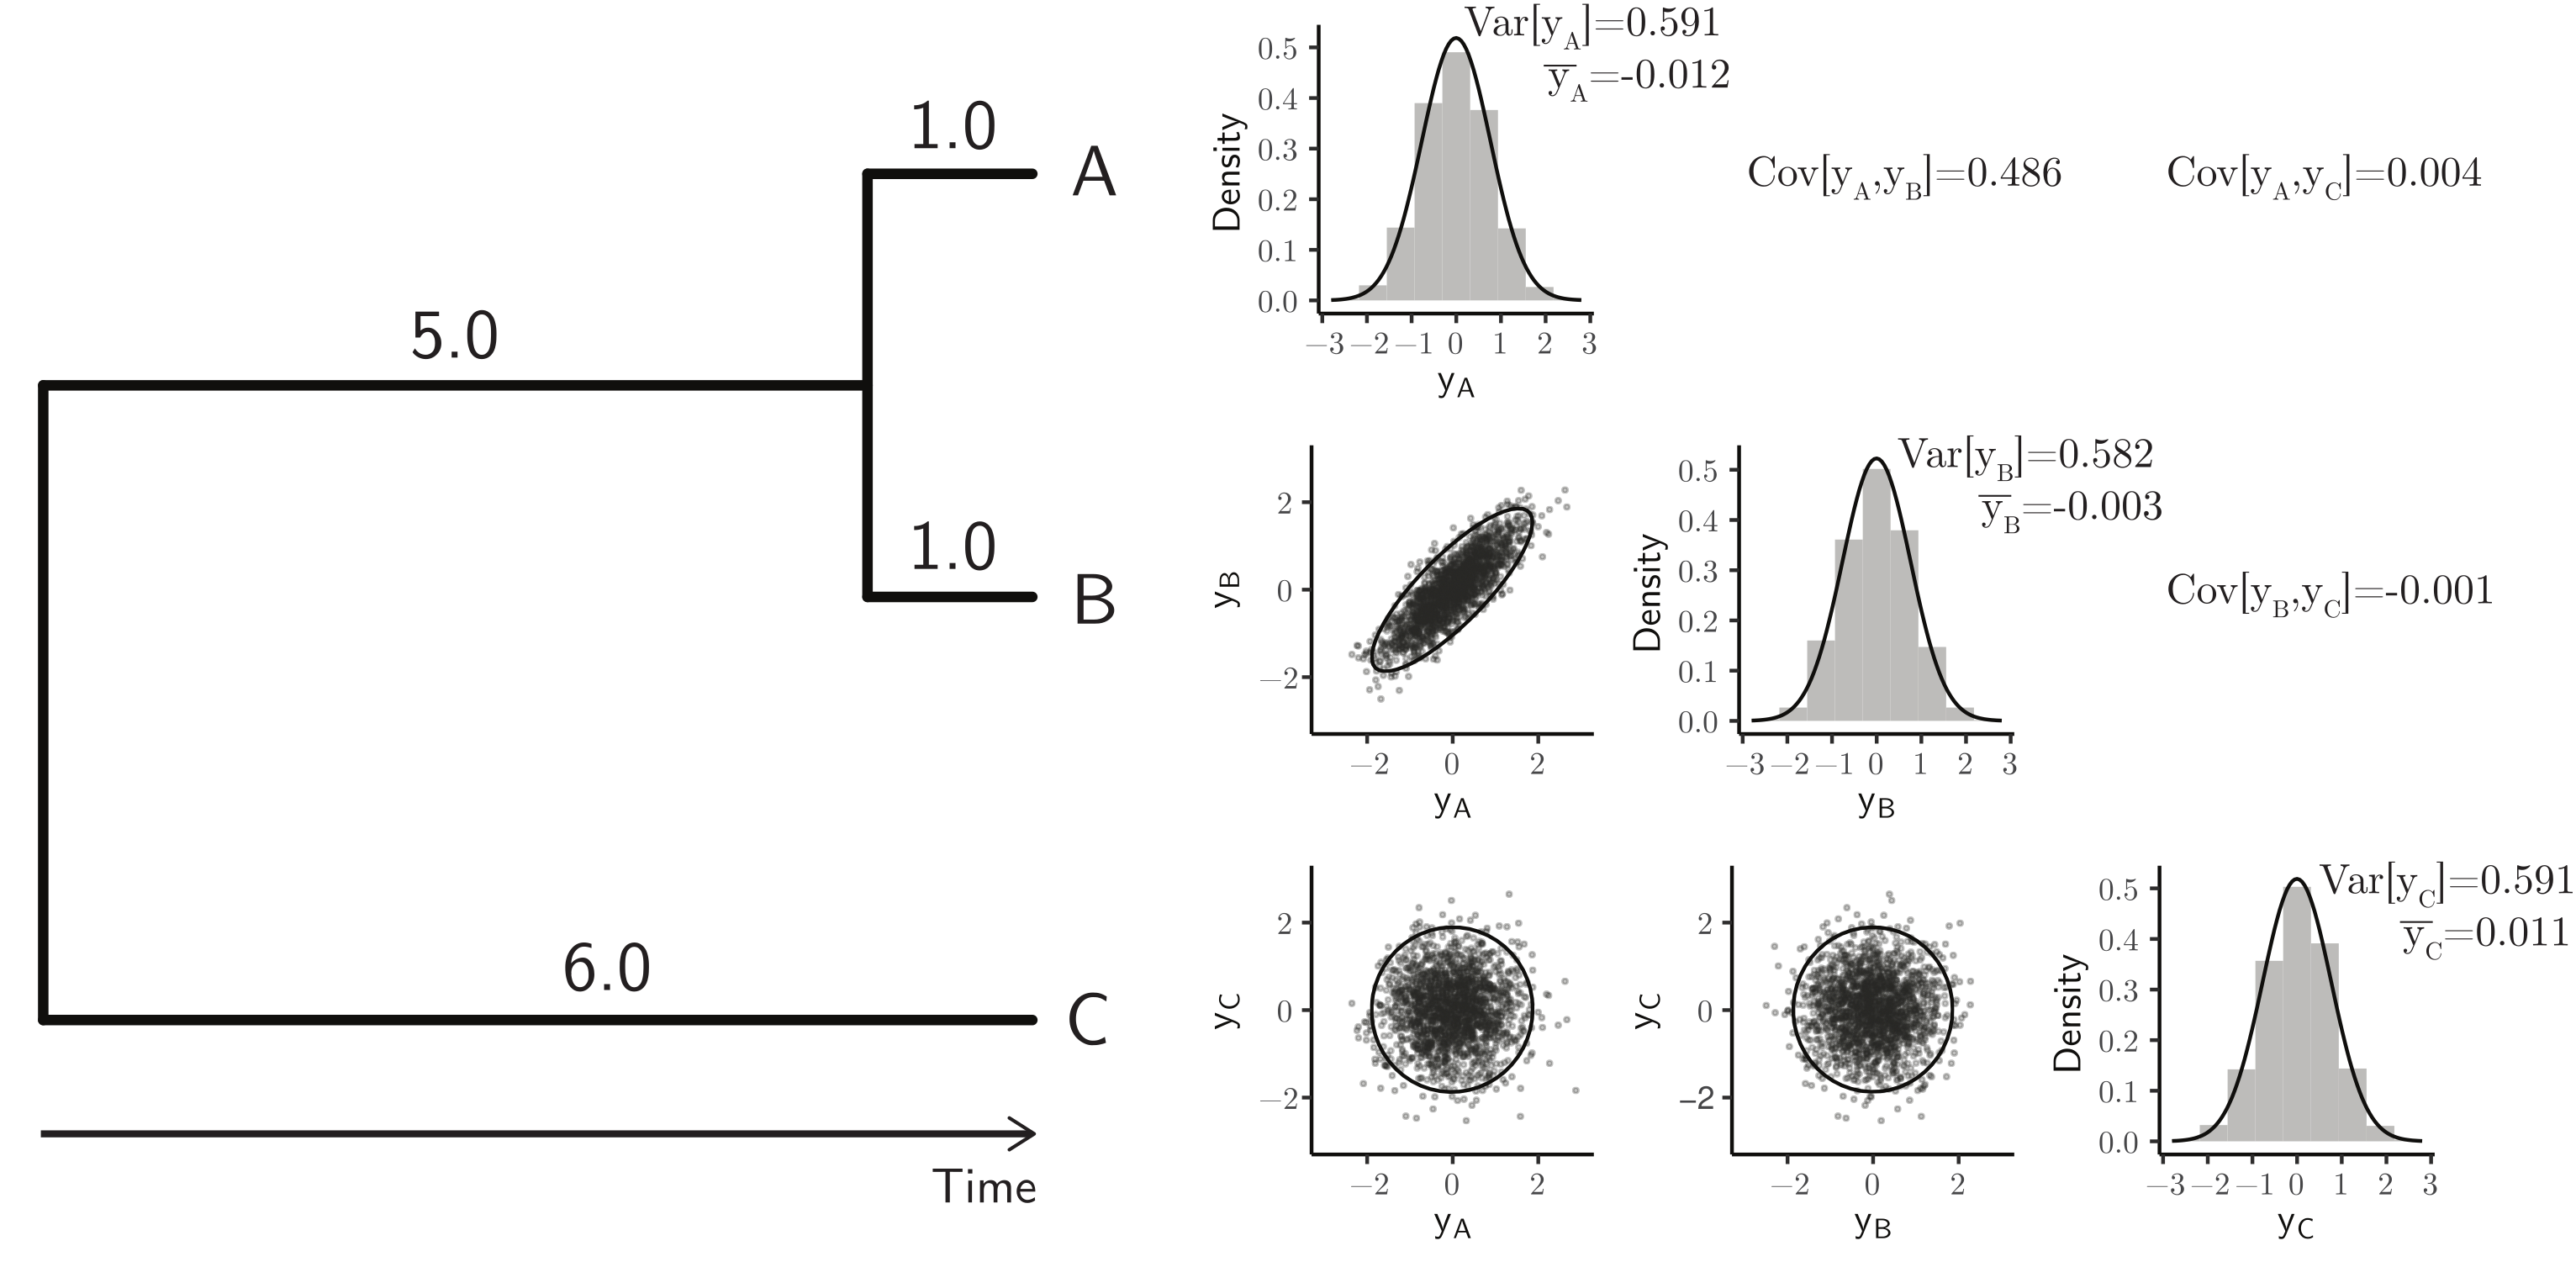
\includegraphics[width=11cm]{../figures/phylobm_exp_vcv.pdf}
  \caption{A sample of 1000 draws from a MVN distribution, each representing the evolutionary trajectory of one continuous trait along the species tree on the left.
    The root trait value, $\boldsymbol{y_0}$, and the evolutionary rate of the process, $r$, were set to 0.0 and 0.1, respectively.
    The panel on the right shows histograms of 1000 trait values sampled from the MVN for each species, as well as their covariation.}
  \label{fig:bmsim}
\end{figure}

More rigorously, one can follow the method described in the main text -- as we do in what follows -- and verify that those expectations fall within their 95\%-confidence intervals 95\% of the time, as calculated from a large number of samples (Supplementary Fig. \ref{supfig:bmsimcis} and Supplementary Table \ref{suptab:bmsimcis}).
Here, we will verify that the expected value of certain summary statistics (given a specific combination of parameter values) falls within its $\alpha$-confidence intervals approximately $\alpha$\% of the time.
We will build confidence intervals about statistics calculated from several PhyloBM samples of size 10,000, and then ask if the ``population'' value of  a statistic -- given by the parameters of the multivariate normal sampling distribution -- is contained within its confidence interval frequently enough.

For summary statistics, we pay attention to the trait value's (i) species mean, (ii) species variance, (iii) among-species covariance, and (iv) among-species correlation coefficient.
Supplementary figure \ref{supfig:bmsimcis} shows one hundred confidence intervals for each of these statistics, under multivariate normal $\text{MVN}(\boldsymbol{y_0},r\boldsymbol{T})$, where $\boldsymbol{y_0}=\{0,0,0\}$, $r=0.1$ and $\boldsymbol{T}$ is given by the tree in Fig. 2 in the main text.
Supplementary table \ref{suptab:bmsimcis} summarizes how often each statistic fell within its 95\%-confidence interval.
These results indicate the PhyloBM simulator produces appropriate confidence intervals and behaves as expected.

\begin{figure}
  \centering
  \includestandalone[width=14cm]{../figures/phylobm_exp_vcv_cis}
  \caption{One hundred 95\%-confidence intervals (blue and red lines) built for four different summary statistics, when validating a phylogenetic Brownian motion model simulator.
    Red lines represent intervals that do not contain the value expected under the MVN sampling distribution defined by a bifurcating three-taxon phylogenetic tree.
    Summary statistics include each leaf's character-value mean (top row) and variance (second row from the top), as well as pairwise (leaf) character-value co-variances (third row from the top) and correlations (bottom row).}
  \label{supfig:bmsimcis}
\end{figure}

\begin{table}[h]
  \caption{The number of times $k$ that a summary statistic was contained within its corresponding 95\%-confidence interval.
    Each statistic was calculated from 100 datasets of size 10,000 simulated under the PhyloBM model described in the text.}
  \label{suptab:bmsimcis}
  \centering
  \begin{tabular}{ ccc }
    \hline
    Statistic & Species $s$ (and $v$)& $k$\\
    \hline  
    \rowcolor{gray!10}                      & A & 95\\
    \rowcolor{gray!10} $\text{E}[y_s]$      & B & 97\\
    \rowcolor{gray!10}                      & C & 98\\
                                            & A & 93\\
                       $\text{Var}[y_s]$    & B & 97\\
                                            & C & 97\\
    \rowcolor{gray!10}                      & A and B & 95\\
    \rowcolor{gray!10}$\text{Cov}[y_s,y_v]$ & A and C & 95\\
    \rowcolor{gray!10}                      & B and C & 97\\
                                            & A and B & 96\\
                      $\text{Cor}[y_s,y_v]$ & A and C & 96\\
                                            & B and C & 97\\
    \hline
  \end{tabular}
\end{table}

\newpage
\section{Model validation with rejection sampling: a simple example}
\label{sec:supp_toy}

In this section, we experiment with a simple hierarchical Gaussian (toy) model to further examine the effect of rejection sampling in coverage validation and
rank-uniformity validation (RUV).
This experiment is motivated by results described in the main text, namely, the model in scenario 3 (Fig. 1, with extreme rejection sampling) passing coverage validation but not RUV.

Let us devise the following data-generating process for obtaining different levels of model misspecification:

\begin{align*}
 \mu & \sim \operatorname{Normal}\left(0, 1\right)T[t, ],\\
  y_1, \ldots, y_K & \overset{\text{iid}}{\sim} \operatorname{Normal}\left(\mu, 1\right),
\end{align*}
where $K$ is the sample size, and notation $T[, t]$ indicates the distribution is truncated \textbf{below} at $t \in \mathbb{R}$, i.e.,
\begin{equation*}
    \pi_{t}(\mu) = \frac{\phi(\mu)}{1 - \Phi(t)} \mathbb{I}(\mu > t).
\end{equation*}
and $\phi$ and $\Phi$ are the pdf and CDF of a standard normal, respectively.
Here, $\mu$ and $y_1, \ldots, y_K$ correspond to $\theta_i$ and $d_i$ in Fig. 4 (main text), respectively.

Inference is then done under the misspecified model
\begin{align*}
 \mu & \sim \operatorname{Normal}\left(0, 1\right),\\
  y_1, \ldots, y_K & \overset{\text{i.i.d.}}{\sim} \operatorname{Normal}\left(\mu, 1\right).
\end{align*}
It is well-known that:
\begin{equation}
\label{eq:toy_normal_posterior}
    \mu \mid y_1, \ldots, y_K \sim \operatorname{Normal}\left( \frac{\sum_{k = 1}^K y_k}{K + 1},  \frac{1}{K + 1} \right),
\end{equation}
i.e., the posterior is known in closed-form so MCMC is not required and one can sample directly and independently from it.
One can thus control how extreme the model misspecification will be during inference by increasing $t$.
Here we explore $t =  \{0, 1, 1.5\}$ and $K = \{5, 10 , 50\}$ in order to show how the method behaves in various misspecification scenarios.
We ran $n=1000$ replications of the experiment, draw $200$ i.i.d. samples directly from the posterior in (\ref{eq:toy_normal_posterior}).

The resulting rank histograms (Supplementary Fig.~\ref{supfig:ruv_normal_toy}) show how the posterior consistently underestimates the true mean, as indicated by a pattern of ranks bunching up towards the right-hand side of the histogram.
The pattern is clearer in situations where the evidence in the data is weaker (e.g., when $K$ is small), and the effect of the prior on the posterior is stronger.
Moreover, the misspecification becomes more apparent the larger $t$ is, that is, the more extreme the misspecification becomes.

It is worth noting a couple of things.
First, unlike what we observed and reported for the model in the main text, coverage validation does suggest an incorrectly specified model for certain combinations of $t$ and $K$ (Supplementary Table 2).
Second, when the truncation is less extreme ($t = 0$) and there is a substantial amount of data ($K = 50$), RUV fails to detect any problems.
This is an important insight about validation protocols: their sensitivity is context-dependent, and responds to the combination of model and data regime.

\begin{figure}[!ht]
   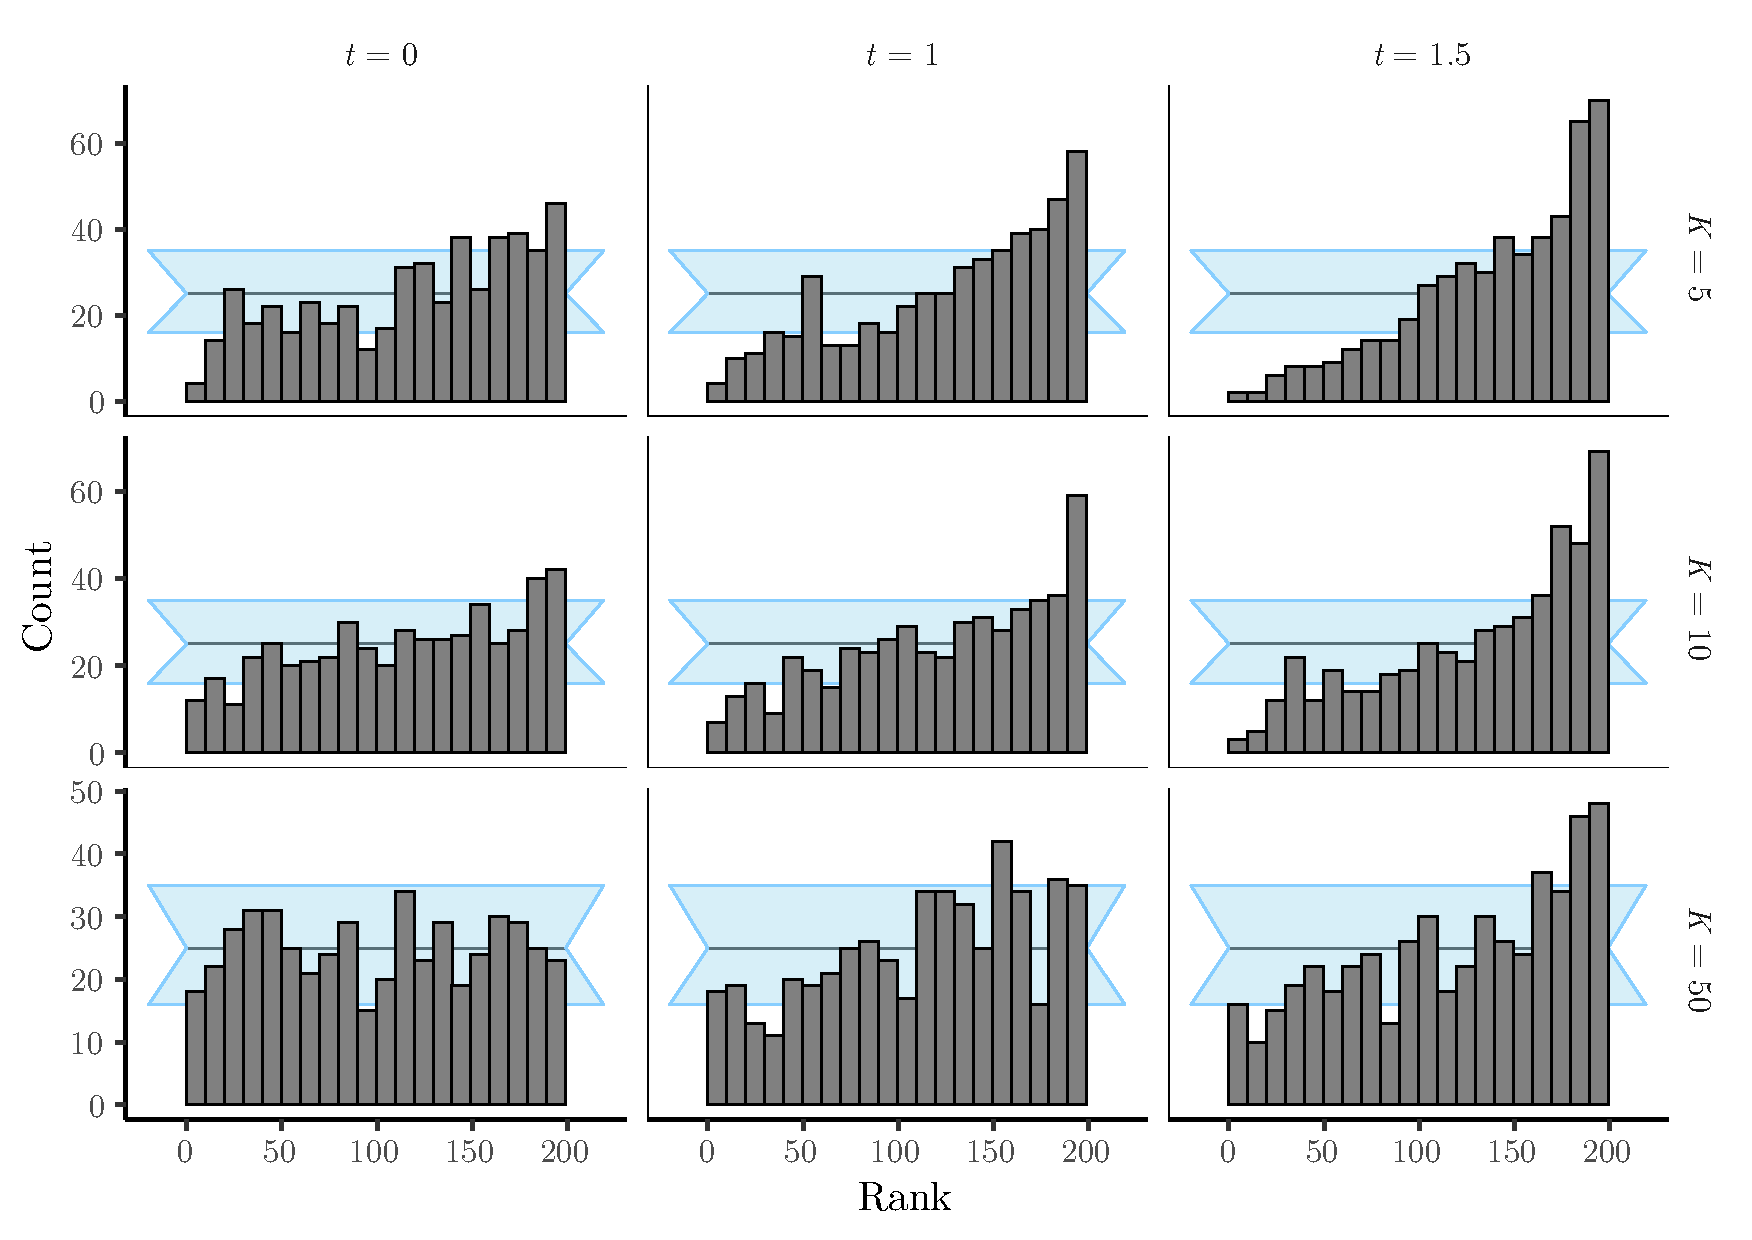
\includegraphics[width=\linewidth]{../figures/sbc_normal_manual.pdf}
  \caption{Rank-uniformity validation (RUV) of the hierarchical Gaussian toy model.
  We show the rank histograms in three misspecification scenarios ($t$
  is 0.0, 1.0 or 1.5) and three data regimes ($K$ is 5, 10 or 50).
  Results are based on $n=1000$ replicates of $L= 200$ i.i.d. draws each.
  Horizontal black lines show the expected count for each rank (the same for all ranks due to uniformity), and the light-blue bands represent the 95\%-confidence interval for the counts.
    }
  \label{supfig:ruv_normal_toy}
\end{figure}

\begin{table}[!h]
\caption{Coverage results for the 95\%-HPD under the hierarchical Gaussian toy model.
For each combination of truncation ($t$) and data set size ($K$), we show the estimated coverage over $n=1000$ replicates, and whether the coverage procedure passes.
A pass is determined according to table 2 in the main text.
}
\centering
\begin{tabular}{cccc}
  \hline
  Truncation ($t$) & Number of observations ($K$) & Estimated coverage & Pass \\
  \hline
  \rowcolor{gray!10} 0   & 5                      & 0.93               & No     \\
  \rowcolor{gray!10} 1   & 5                      & 0.92               & No     \\
  \rowcolor{gray!10} 1.5 & 5                      & 0.90               & No     \\
                     0   & 10                     & 0.95               & Yes    \\
                     1   & 10                     & 0.91               & No     \\
                     1.5 & 10                     & 0.91               & No     \\
  \rowcolor{gray!10} 0   & 50                     & 0.96               & Yes    \\
  \rowcolor{gray!10} 1   & 50                     & 0.93               & No     \\
  \rowcolor{gray!10} 1.5 & 50                     & 0.93               & No     \\
  \hline
\end{tabular}
\label{suptab:ruv_normal_toy}
\end{table}

\newpage
\section{Validating a phylogenetic model with respect to a phylogenetic tree parameter, $\Phi$}
\label{sec::app::ruv_topology}

Our goal is to evaluate if an inferential implementation of model $\mathcal{M}$, $\text{I}[\mathcal{M}]$, is well-calibrated and correct.
In this section, we will focus on one critical parameter of $\mathcal{M}$: the phylogenetic tree $\Phi$.
We will pay special attention to $\Phi$ while carrying out coverage validation and the RUV procedure.
In practice, this amounts to computing the coverage of $\Phi$ and the rank distribution of this parameter in comparison to its posterior samples.

What feature of $\Phi$ should one use when calculating coverage and ranks?
Because of the nature of tree space, summarizing and comparing phylogenetic trees with univariate measures is not a trivial task.
The key to an effective validation effort is to choose a functional that reflects relevant estimators of the quantity of interest, in our case, $\Phi$.
Fortunately, it is possible to exploit the metric nature of tree space and compute quantities both from a sampled phylogenetic tree $\phi$ -- i.e., the ``true'' tree simulated during the validation process -- as well as distances with respect to a reference phylogeny $\phi_0$.
We summarize some of these distances in supplementary table \ref{suptab:dists}.

\begin{table}[h]
  \caption{Metrics (functionals) for investigating model correctness in phylogenetic tree space. $\phi$ is a (phylogenetic tree) sample of $\Phi$, sampled from a tree model (e.g., a Yule process).
  $\phi_0$ is a reference tree to which $\phi$ and its posterior samples (see Algorithm 1 and the RUV section in the main text) are being compared, with respect to any of the metrics in the table.
  For the KC metric, the parameter ($\omega$) controls the balance between topological and branch length information, and was set at $\omega = 0.5$. }
  \label{suptab:dists}
  \centering
  \begin{tabular}{ l|c|c }
    \hline
    \multicolumn{1}{c|}{Metric} & Notation & Ref. \\
    \hline  
    \rowcolor{gray!10}The largest branch length in $\phi$ & $\text{LB}(\phi)$ & N/A\\
    The length of $\phi$ (the sum of all branch lengths) & $\text{LEN}(\phi)$ & N/A\\
    % \rowcolor{gray!10}The length of the external branch leading to taxon $s_1$ & $\text{T}_1(\phi)$ & N/A\\
    \rowcolor{gray!10}The difference between the largest and smallest branch length of $\phi$ & $\text{R}(\phi)$ & N/A\\
    The Robinson-Foulds distance between $\phi$ and $\phi_0$ & $\text{RF}_0(\phi)$ & \citep{foulds81}\\
    \rowcolor{gray!10}The Kendall-Coljin distance between $\phi$ and $\phi_0$ & $\text{KC}_0(\phi;\omega)$ & \citep{Kendall2016}\\
    The Billera-Holmes-Vogtman distance between $\phi$ and $\phi_0$ & $\text{BHV}_0(\phi)$ & \citep{Billera2001}\\
    \hline
  \end{tabular}
\end{table}

In the case of tree-space distance metrics, we must slightly modify our RUV procedure (Algorithm 1).
The key difference is the sampling of a reference phylogenetic tree, $\phi_0$, prior to the simulation of the $n$ i.i.d. $\Phi$ samples, $\boldsymbol{\phi}=\{\phi_i: 1 \leq i \leq n\}$.
Given a reference tree $\phi_0$, each sampled $\phi_i$ and all of its $L$ posterior MCMC samples are then compared to $\phi_0$ with respect to a chosen distance metric.
It is the evaluated distance metric that will underlie the ranking of $\phi_i$ relative to its posterior MCMC samples.
Once ranks are computed, RUV proceeds as usual.
   
\RestyleAlgo{ruled}
\SetKwComment{Comment}{/* }{ */}

\begin{algorithm}[h]
  \DontPrintSemicolon
  \SetKwFunction{GenRefTree}{GenerateRefTree}
  \SetKwFunction{InitH}{InitializeHyperparameters}
  \SetKwFunction{SampleNT}{SampleNonTreeParameters}
  \SetKwFunction{SampleTree}{SampleTree}
  \SetKwFunction{SampleData}{SampleData}
  \SetKwFunction{Distance}{CalculateDistance}
  \SetKwFunction{MCMC}{MCMC}
  \SetKwFunction{Rank}{GetRank}
  \SetKwFunction{Pass}{IsRankDistributionUniform}
  \caption{Algorithm for carrying out a rank-uniformity validation procedure with respect to the phylogenetic tree parameter $\Phi$.
    Parameters $\boldsymbol{\theta}$ include both the tree parameter, $\theta_\Phi$, and non-tree (scalar) parameters, $\boldsymbol{\theta}_{\text{s}}$.
    Data $\boldsymbol{d}$ represents the output of an evolutionary process taking place along the phylogenetic tree (e.g., a continuous-time Markov chain modeling DNA substitutions).}
  \label{alg:sbcphylo}
  $n \gets 100$\; \Comment*[r]{Number of data sets to simulate}
  $\theta_{\mathcal{H}} \gets$ \InitH{}\; \Comment*[r]{Hyperparameters initialized to constant values}
  $\boldsymbol{\theta}_0 \gets$ \SampleNT{$\theta_{\mathcal{H}}$}\; \Comment*[r]{$\boldsymbol{\theta}_0 \sim f_\Theta(\cdot)$, with $\boldsymbol{\theta}_0 = \{\theta_{\Phi,0},\boldsymbol{\theta}_{\text{s},0}\}$}
  $\phi_0 \gets$ \SampleTree{$\theta_{\Phi,0}$}\; \Comment*[r]{$\phi_0 \sim f_{\Phi|\Theta_{\Phi}}(\cdot|\Theta_\Phi=\theta_{\Phi,0})$}
  \For{$i \gets 1$ \KwTo $n$} {
    $\boldsymbol{\theta}_i \gets$ \SampleNT{$\theta_{\mathcal{H}}$}\; \Comment*[r]{$\boldsymbol{\theta}_i \sim f_\Theta(\cdot)$, with $\boldsymbol{\theta}_i = \{\theta_{\Phi,i},\boldsymbol{\theta}_{\text{s},i}\}$}
    $\phi_i \gets$ \SampleTree{$\theta_{\Phi,i}$}\; \Comment*[r]{$\phi_i \sim f_{\Phi\mid \Theta_\Phi}(\cdot|\Theta_\Phi=\theta_{\Phi,i})$}
    $d_i \gets$ \SampleData{$\phi_i,\boldsymbol{\theta}_{\text{s},i}$}\; \Comment*[r]{$d_i \sim f_{D\mid \Phi,\boldsymbol{\Theta}_\text{s}}(\cdot|\Phi=\phi_i,\boldsymbol{\Theta}_{\text{s}}=\boldsymbol{\theta}_{\text{s},i})$}
    $\boldsymbol{\theta}'_i \gets$ \MCMC{$f_{D|\boldsymbol{\Theta}}(d_i|\boldsymbol{\Theta}=\boldsymbol{\theta}_i)f_{\boldsymbol{\Theta}}(\boldsymbol{\theta}_i)$}\; \Comment*[r]{$\boldsymbol{\theta}'_i = \{\boldsymbol{\theta}_i^j: 1 \leq j \leq L\}$, where $L$ is the number of MCMC samples}
    $\bar{\delta}_i \gets$ \Distance{$\phi_0, \phi_i$}\; \Comment*[r]{According to a distance metric of choice}
    $\boldsymbol{\delta}_i^j \gets$ \Distance{$\phi_0, \phi_i^j$}\; \Comment*[r]{$\boldsymbol{\delta}_i = \{\delta_i^j: 1 \leq j \leq L\}$}
    $r_i \gets$ \Rank($\bar{\delta}_i, \boldsymbol{\delta}_i^j$)\; \Comment*[r]{$r_i = \sum\limits_{j=1}^L \mathbb{I}(\delta^j_i < \bar{\delta_i})$}
  }
  \If{\Pass{$\boldsymbol{r}$}}{
    \Return \textbf{true}
  }
  \Else {
    \Return \textbf{false}
  }
  \label{alg:sbc}
\end{algorithm}

  % \begin{enumerate}
  %   \setcounter{enumi}{-1}

  % \item Generate a reference tree from the prior $\bar{\Phi}_0  \sim f_T(\Phi | \boldsymbol \theta_\Phi)$; 

  %   \textbf{for} each iteration in 1:N, \textbf{do}:
    
  % \item Generate $\bar{\Phi} \sim f_T(\Phi | \boldsymbol \gamma)$;
  % \item Compute the distance $\bar{\delta} = d_\sigma(\bar{\Phi},\bar{\Phi}_0)$ according to the metric of choice;
  % \item Generate some (aligment) data $\tilde{d} \sim f_{D\mid\Phi}(d | \bar{\Phi}, \boldsymbol\alpha)$;
  % \item Draw\footnote{Sometimes approximately, using MCMC or variational methods.} $\boldsymbol \Phi_s = \{\Phi_s^{(1)}, \Phi_s^{(2)}, \ldots, \Phi_s^{(L)}\}$ from the posterior $f_{\Phi\mid D}(\Phi | \tilde{d})$;
  % \item Compute distances $\boldsymbol \delta_s = \{ \delta_1, \delta_2, \ldots, \delta_L \}$  with $\delta_i = d_\sigma(\Phi_s^{(i)}, \bar{\Phi}_0)$;
  % \item Compute the rank $r(\boldsymbol\delta_s, \bar{\delta}) = \sum\limits_{i=1}^L \mathbb{I}(\delta_i < \bar{\delta})$.
  % \end{enumerate}

\begin{figure}
  \centering
  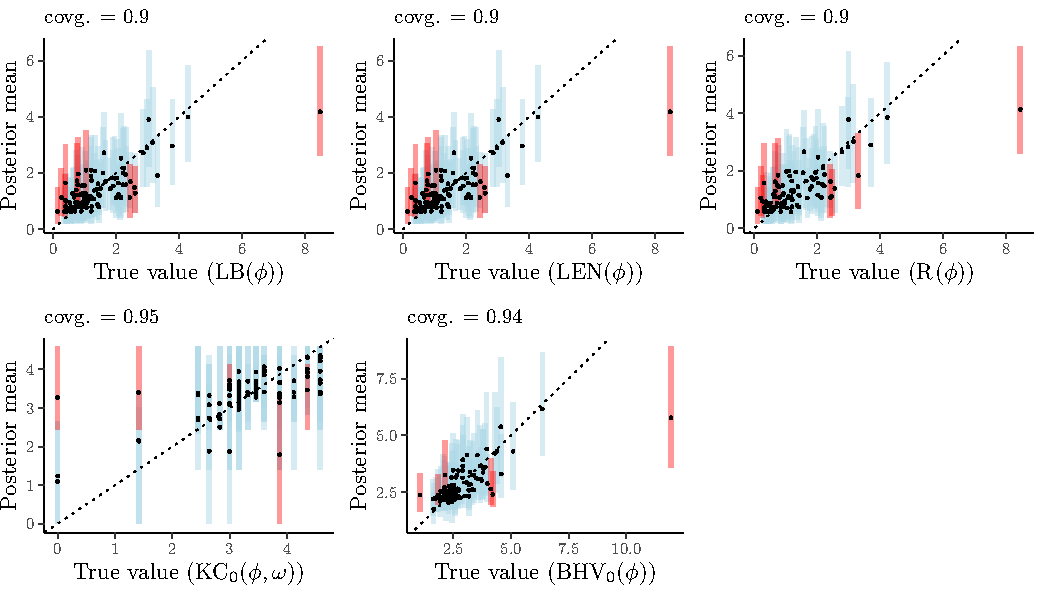
\includegraphics[width=\linewidth]{../figures/tree_stats_coverage_manual.pdf}
   \caption{Coverage validation of a phylogenetic model, focusing on the phylogenetic tree parameter (see Supplementary Table \ref{suptab:dists} for a description of the different distance metrics).}
   \label{supfig:treecov}
 \end{figure}
 
\begin{figure}
  \centering
  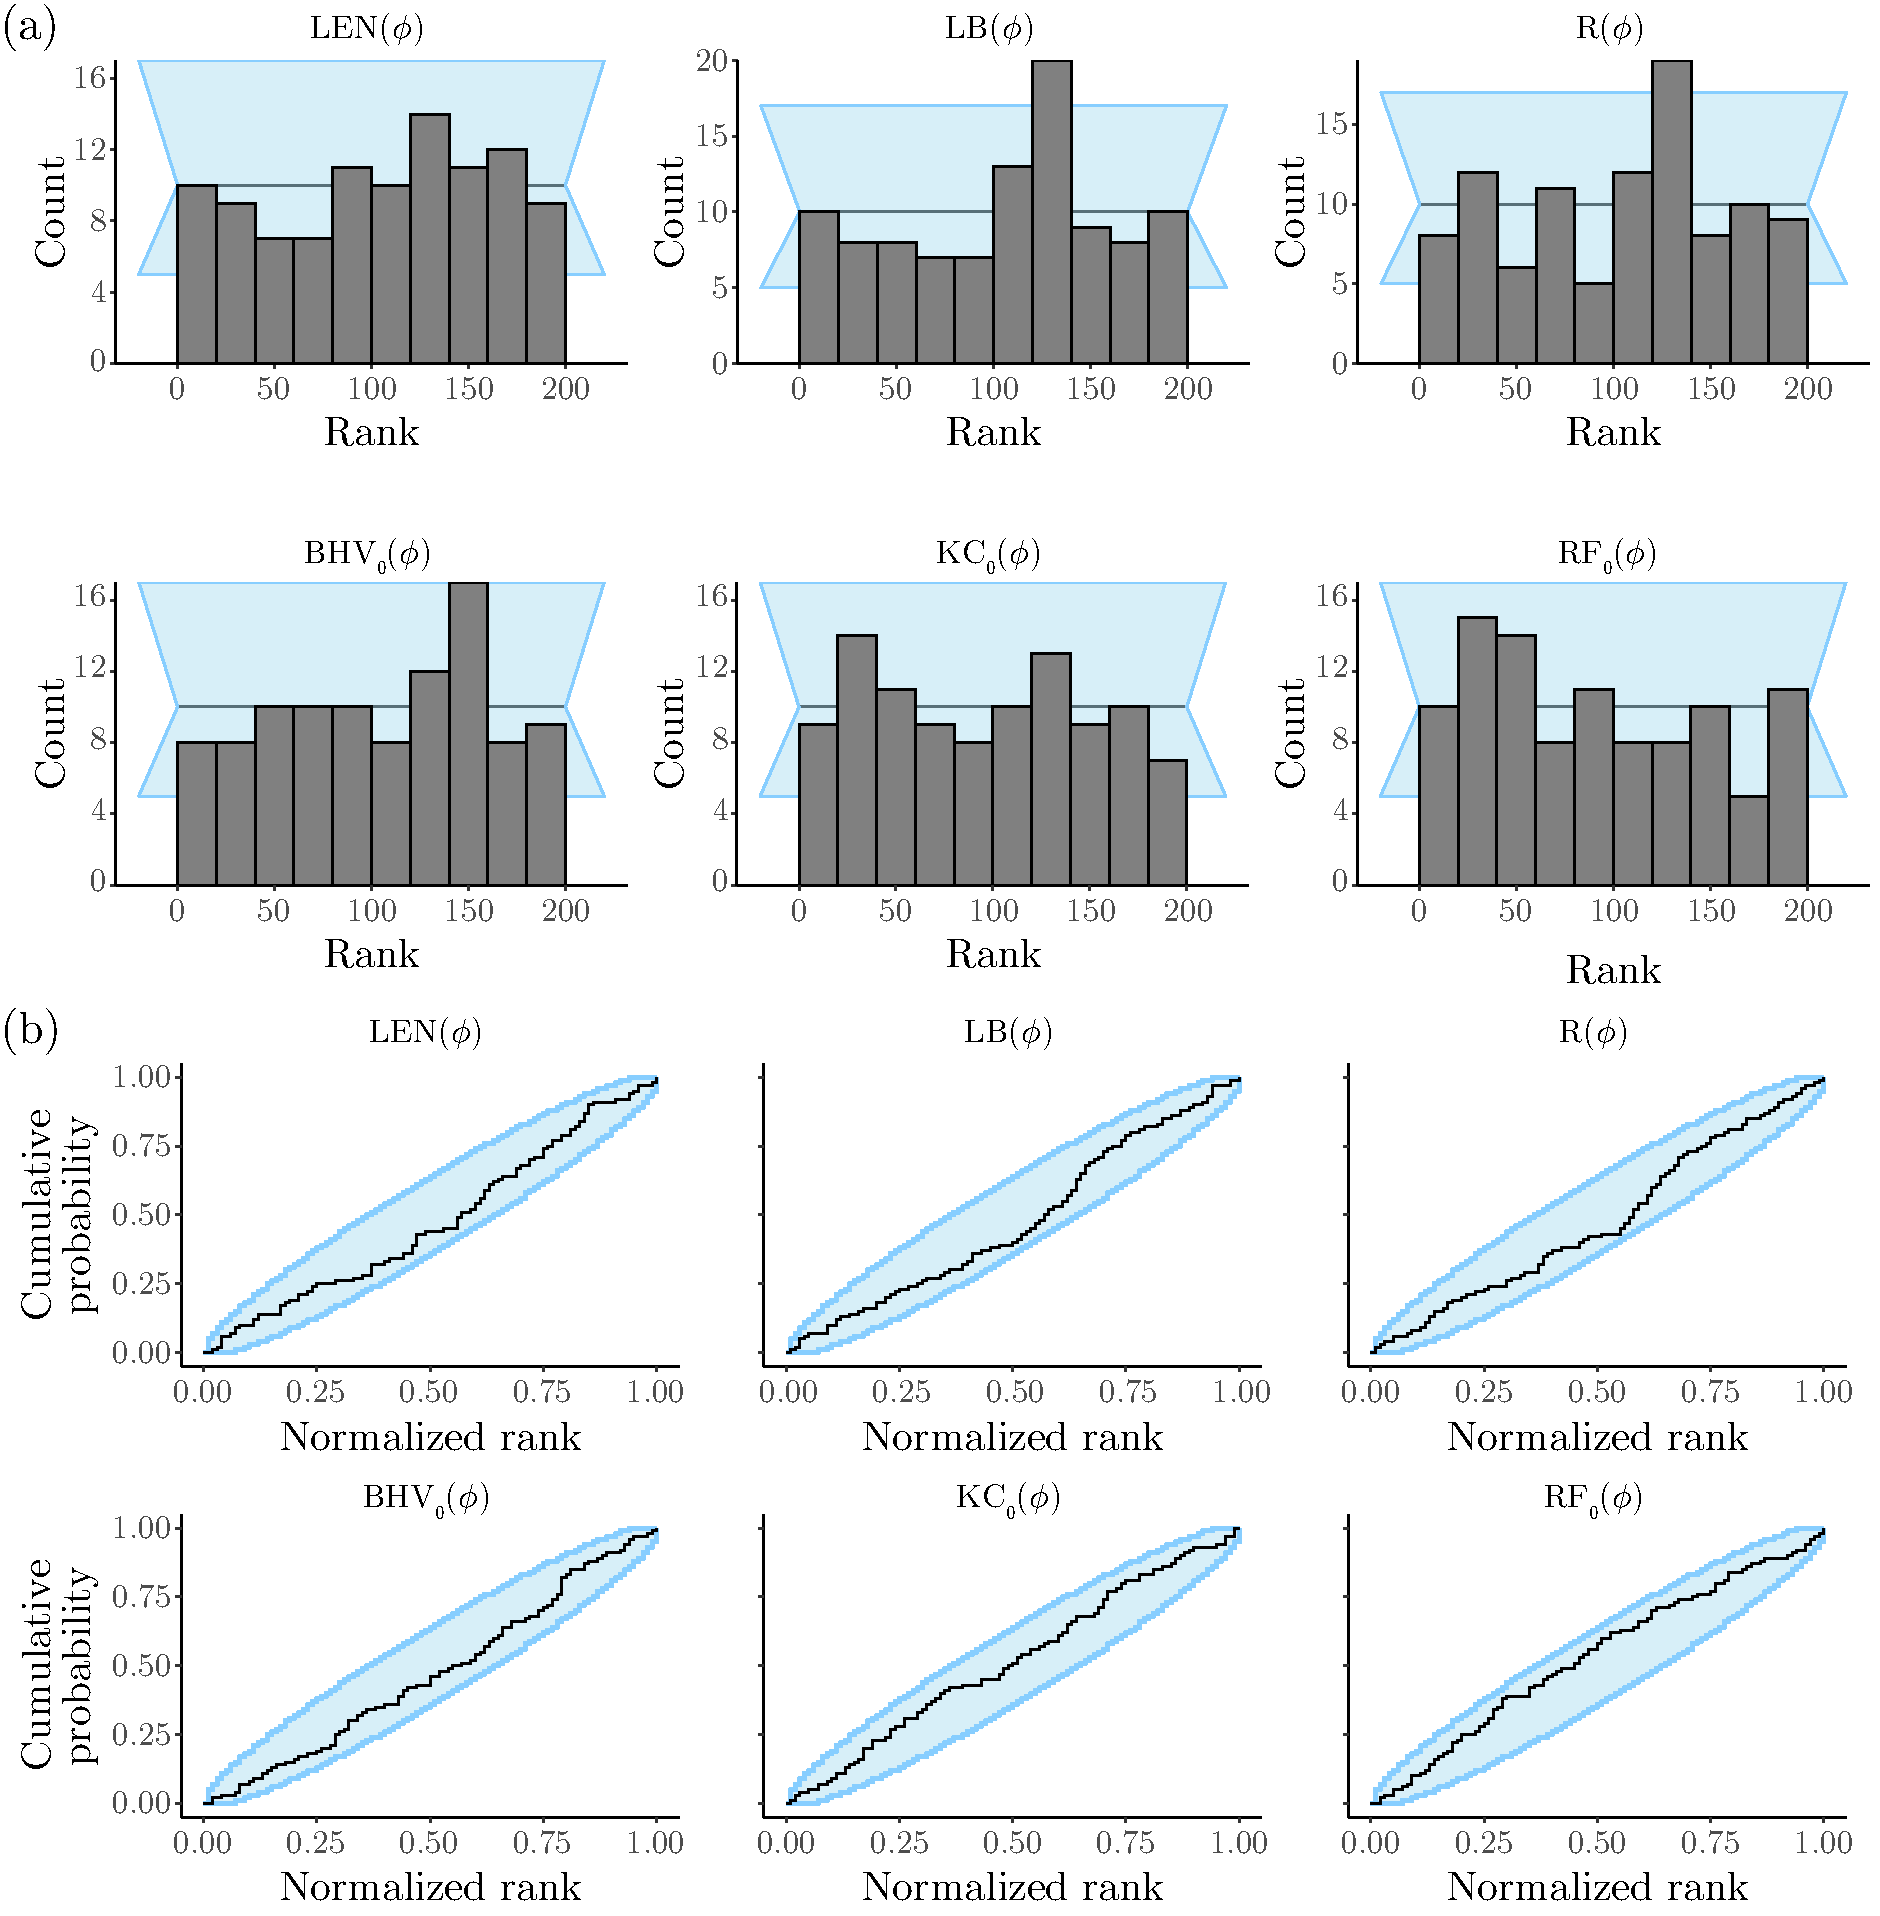
\includegraphics[width=\linewidth]{../figures/ruv_coalescent_manual.pdf}
  % \vspace{0pt}
  % \begin{subfigure}[t]{\textwidth}
  %   \caption{}
  %   \centering
  %   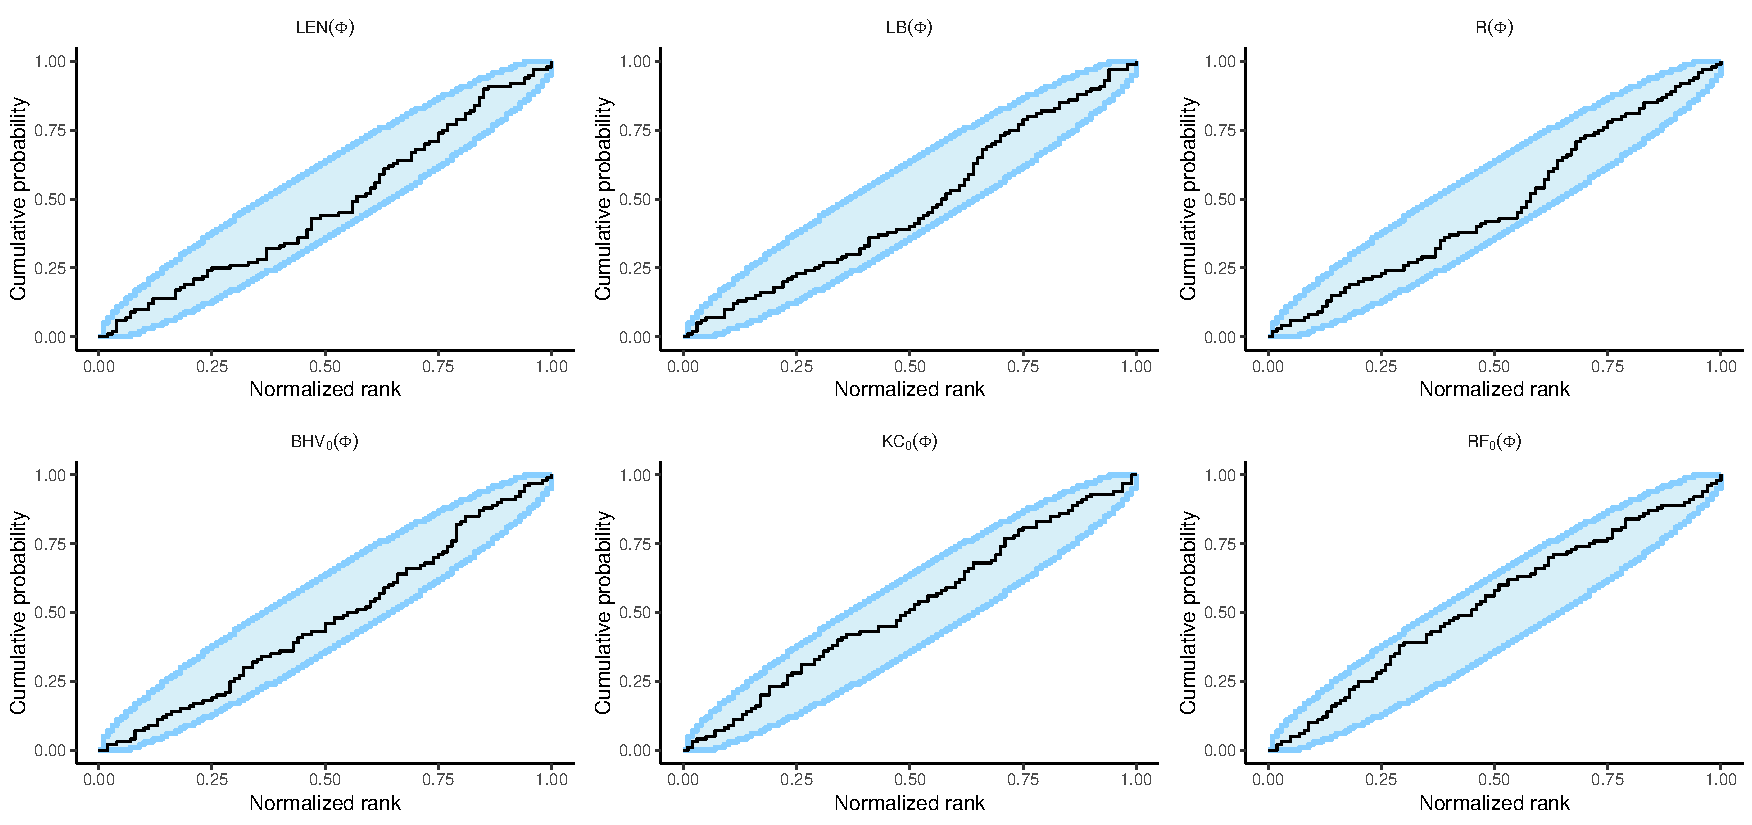
\includegraphics[scale=0.5]{../figures/ruv_coalescent_ecdfs.pdf} 
  % \end{subfigure}
  % \vspace{0pt}
  % \hspace{1cm}
  % \begin{subfigure}[t]{\textwidth}
  %   \caption{}
  %   \centering
  %   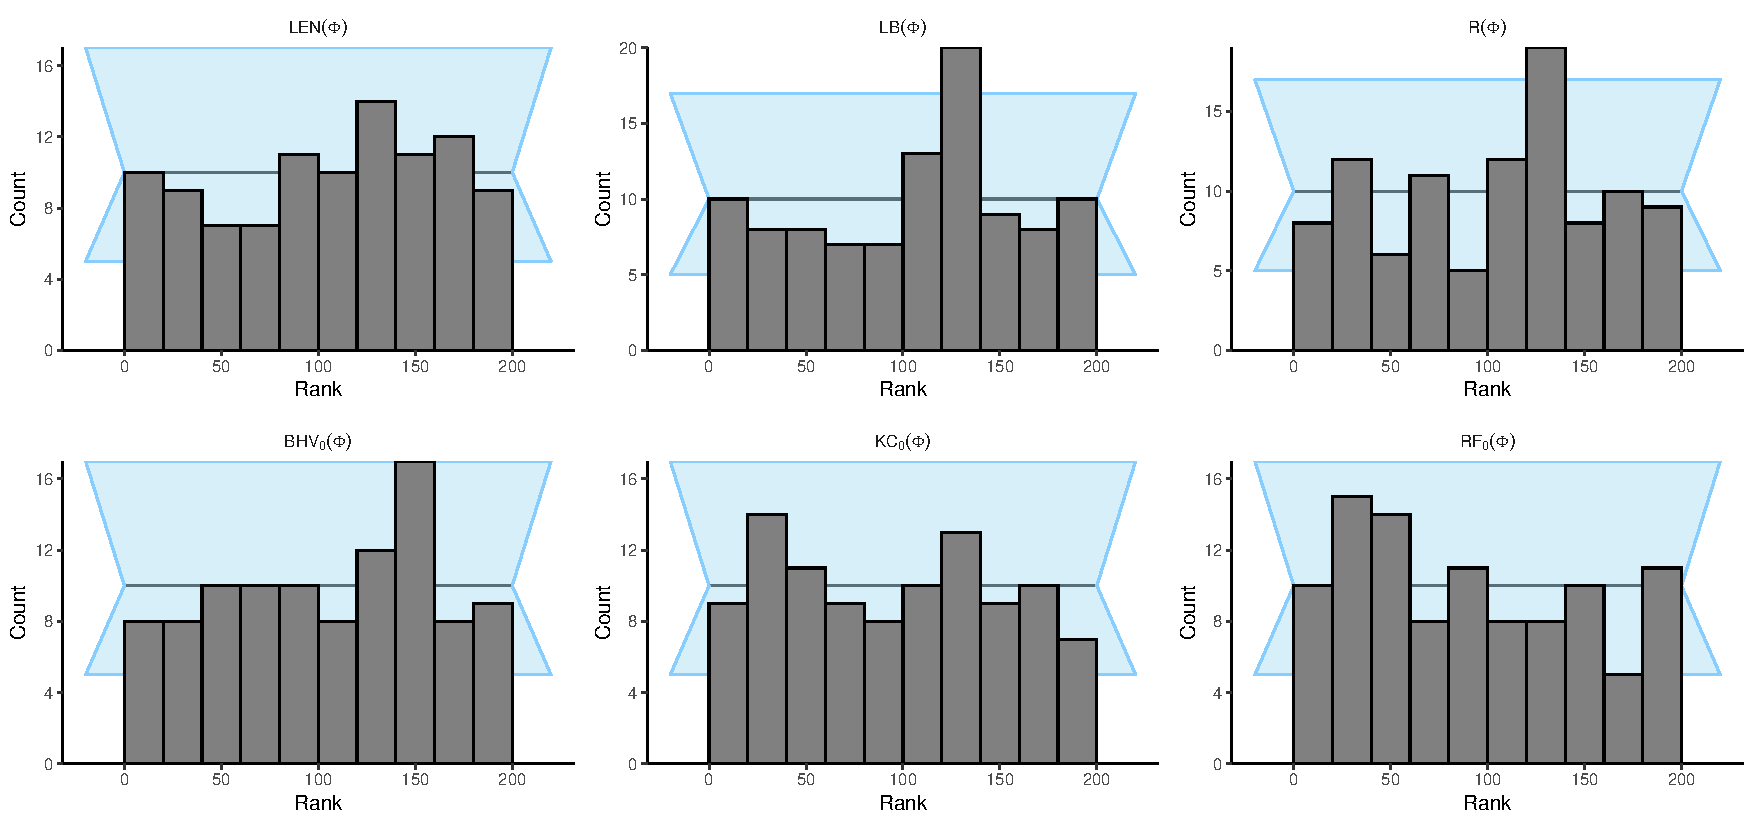
\includegraphics[scale=0.5]{../figures/ruv_coalescent_histograms.pdf}    
  % \end{subfigure}
  % \hfill
   \caption{Rank-uniformity validation (RUV) of a phylogenetic model, focusing on the phylogenetic tree parameter (see Supplementary Table \ref{suptab:dists} for a description of the different distance metrics).
     (a) Rank distribution for each metric.
     (b) Empirical cumulative distribution function (ECDF) for each metric.
   }
   \label{supfig:ruv}
\end{figure}

% \begin{figure}
%  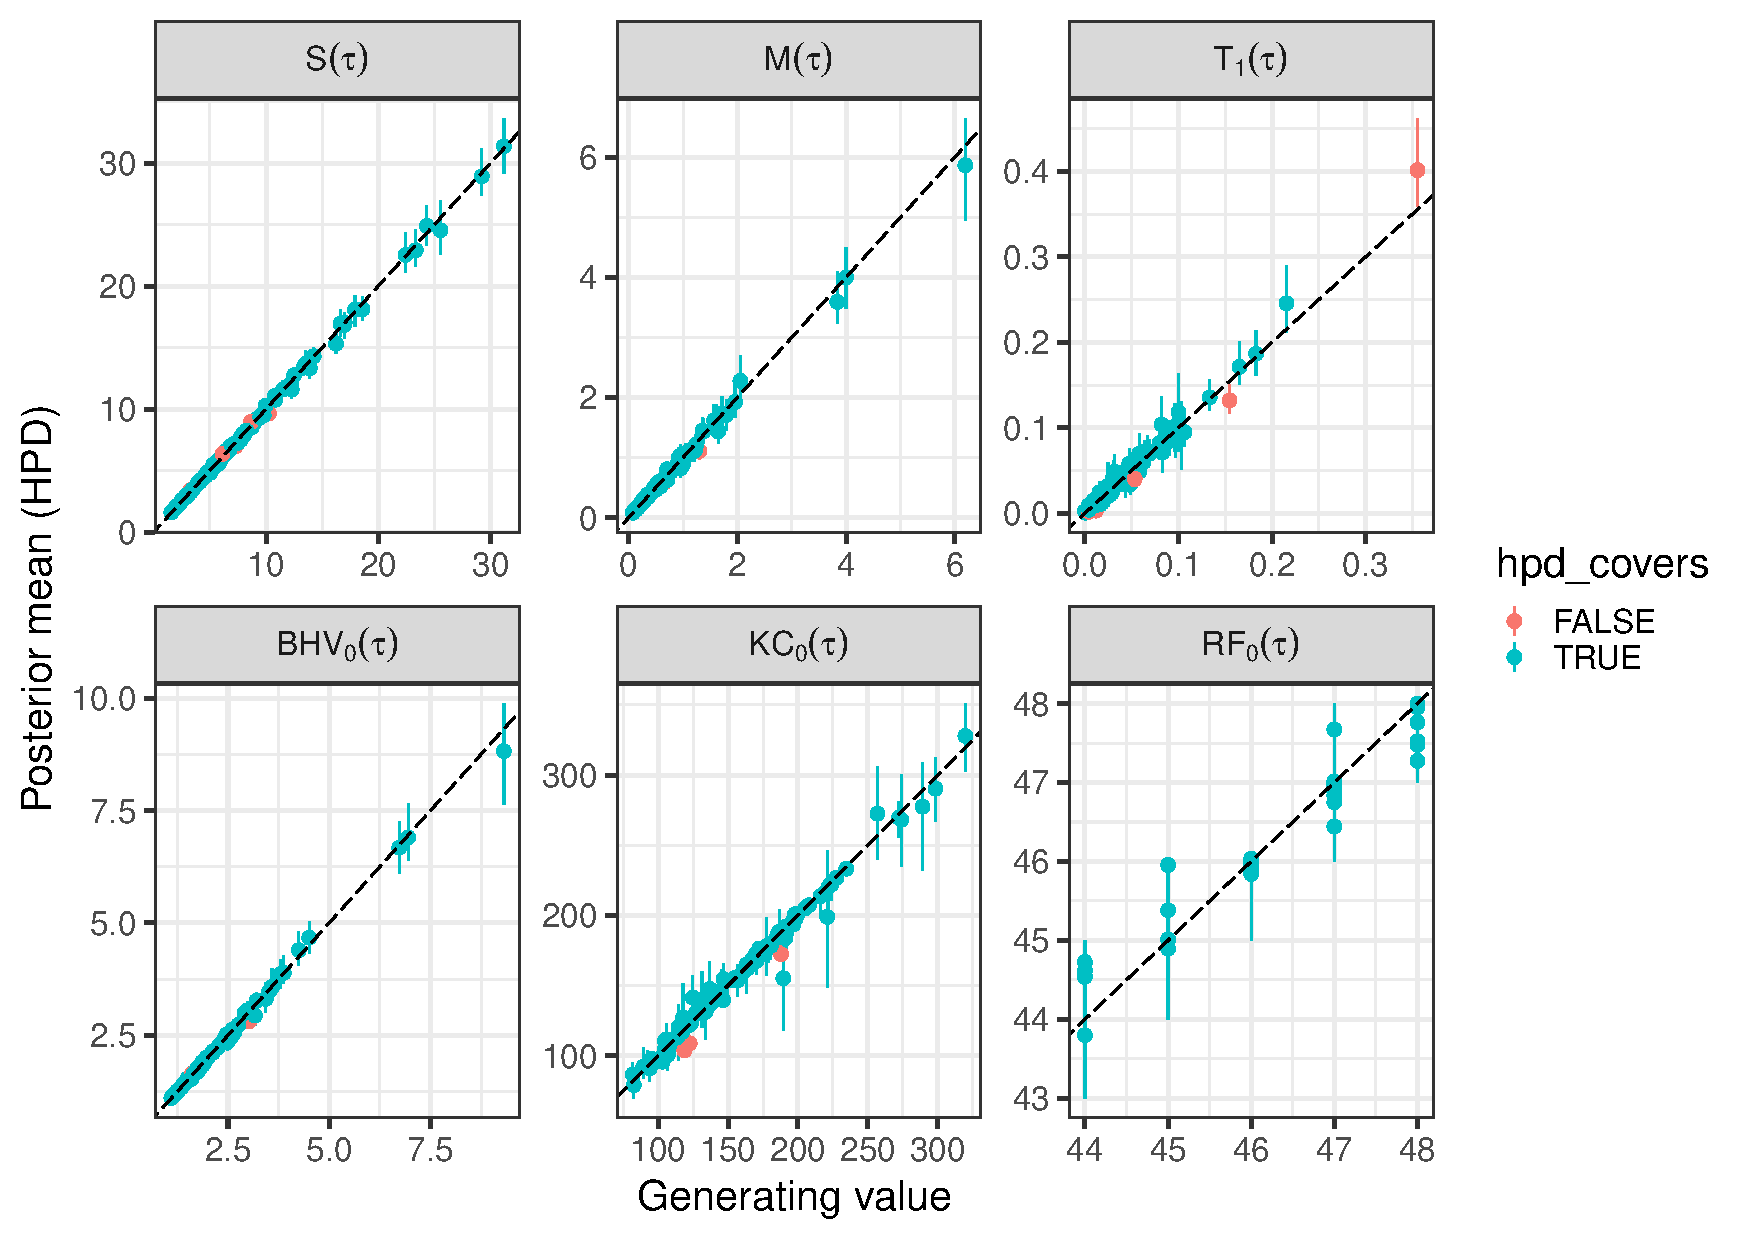
\includegraphics[width=\textwidth]{../figures/coverage.pdf}
%     \caption{Coverage for different functionals in validation experiment.
%         % rank-uniformity validation.
%       Posterior means are represented by point and 95\% HPDs by bars.
%       Red dots and lines show intervals that failed to include the
%       generating value, whilst blue ones show those that did include
%       the simulated ``truth''.}
%   \label{supfig:phylo_calibration}
% \end{figure}

Supplementary figures \ref{supfig:treecov} and \ref{supfig:ruv} summarize the coverage and RUV results, respectively, for the metrics listed in supplementary table \ref{suptab:dists}, when the model is the simple Kingman's coalescent.
The model consists of a single five-taxon phylogenetic tree parameter, $\Phi$, assuming a known effective population size of 1.0.

We can first verify that our model implementation is well-calibrated with respect to the phylogenetic tree parameter, as shown by appropriate 95\%-HPD-coverage statistics over the different tree metrics (Supplementary Fig. \ref{supfig:treecov}).
The evidence for implementation correctness is enhanced by observing that the ranks for the different metrics are (approximately) uniformly distributed, lying inside their confidence bands (Supplementary Fig. \ref{supfig:ruv}a), and their corresponding ECDFs also lie well inside their confidence ellipses (Supplementary Fig. \ref{supfig:ruv}b).
% Supplementary figure \ref{supfig:phylo_calibration} shows that the HPDs do cover the
% generating metrics with probability compatible with what is expected
% theoretically.
% In this instance, the tests would fail to detect problems with the algorithm.
% These plots can be supplemented with a table showing attained coverage and binomial confidence intervals for this quantity.
% A further advantage of graphically investigating coverage is that one can identify consistent areas for which estimation fails -- e.g. high/low simulated values of a given variable.

In the main text, we also mentioned the possibility of assessing the coverage of a phylogenetic tree's topology; specifically, by looking at the frequency of its clades as a function of their posterior support.
An outcome of this procedure can be seen in supplementary figure \ref{supfig:clade_covg}, for a simple 50-sample Kingman coalescent model.
We propose that the clade frequency diagnostic is further evaluated in two ways.
One can first check that the resulting empirical cumulative distribution function (ECDF) fits that of an appropriately scaled uniform distribution using a Kolmogorov-Smirnov test~\citep{Birnbaum1951}.
Additionally, one can fit a regression model to the attained frequencies against the bin midpoints, and test the null hypothesis that the intercept is zero and the slope is one, rejecting it at the usual confidence levels.

Importantly, there are two considerations we would like to bring to the reader's attention.
First, depending on the starting tree's topology, its number of tips, and the length of the MCMC chain, true clades may never be sampled by chance more frequently than expected.
This could be diagnosed by observing the left-most bar in supplementary figure \ref{supfig:clade_covg} being taller than expected; here, one alternative is to ignore this first bar when carrying out the statistical tests suggested above.

Second, regardless of the simulated phylogenetic signal (with respect to the tree topology) -- irrespective of, e.g., too few, an ideal amount, or too many molecular substitutions in simulated alignments -- the ladder-like pattern in supplementary figure \ref{supfig:clade_covg} should still be observed.
This is because we suggest the count of clades with a given posterior clade support be normalized by the total number of clades with that support: if a very large number of true clades has support close to 0.0 or to 1.0, those counts will be divided by the total count of clades with corresponding support levels.
Trees must have enough tips, however, or a large enough number of trees must be simulated so that all bins, including intermediate support ones, have large enough counts of sampled clades.
Lastly, we emphasize that there is nothing intrinsically wrong with validating a model with a data set void of any signal.
In coverage validation, the prior mean would be recovered for each parameter, and model correctness could still be in principle verified.

\newpage
\section{Proof for coverage validation}
 \label{appendix::sec:proofs}

In this section we provide a mathematical argument that coverage-based validation is sound, i.e., that sampling from the prior, simulating data and then using the same prior for computing the posterior should give Bayesian credible intervals (BCIs) with nominal frequentist coverage.

For a number $n$ of replicates, simulate parameter
  values $\theta_i$, and then given those values, simulate data $d_i$:

\begin{align*}
\theta_i & \sim f_\Theta(\cdot), \\
d_i & \sim f_{D|\Theta}(\cdot | \Theta=\theta_i).
\end{align*}

Now for notational convenience, define $a_i := a(d_i, \alpha)$ as the HPD lower bound and, similarly, $b_i := b(d_i, \alpha)$ as the HPD upper bound.
Recall $I_{\alpha}\left(d_i\right)$ is such that:


\begin{align*}
Q_{d_i}\left(b_i\right) - Q_{d_i}\left(a_i\right) = p_1 - p_2 = \alpha,
\end{align*}

\noindent where $Q_{d}(x)$ is the posterior CDF (conditional on data $d$) and $p_1, p_2 \in (0,1)$, with $p_1 < p_2$.
A natural quantity to compute is:

\begin{align*}
S_n = n^{-1}\sum_{i=1}^n \mathbb{I}\left(\theta_i \in I_{\alpha}\left(d_i\right) \right),
\end{align*}

\noindent i.e., the attained coverage of the Bayesian intervals.

Let $F_U(x) = x$ be the CDF of a $\operatorname{Uniform(0, 1)}$ random variable. 
Now we can consider what happens when the number of simulations grows, i.e., the limit $\lim_{n \to \infty} S_n$.
We may re-write the limit as:

\begin{align*}
\lim_{n \to \infty} S_n &= \lim_{n \to \infty} n^{-1}\sum_{i=1}^n \mathbb{I}\left(\theta_i \in I_{\alpha}\left(d_i\right) \right),\\
&=  \lim_{n \to \infty} n^{-1}\sum_{i=1}^n \left\{ \mathbb{I}\left(\theta_i \leq b_i \right) - \mathbb{I}\left(\theta_i \leq a_i \right) \right\},\\
&=  \lim_{n \to \infty} n^{-1}\sum_{i=1}^n \mathbb{I}\left(\theta_i \leq b_i \right) -  n^{-1}\sum_{i=1}^n\mathbb{I}\left(\theta_i \leq a_i \right),\\
&=  \lim_{n \to \infty} n^{-1}\sum_{i=1}^n \mathbb{I}\left(Q_{d_i}^{-1}\left(\theta_i\right) \leq p_1 \right) -   \lim_{n \to \infty} n^{-1}\sum_{i=1}^n\mathbb{I}\left(Q_{d_i}^{-1}\left(\theta_i\right) \leq p_2 \right),\\
&= F_U(p_1) - F_U(p_2) = \alpha,
\end{align*}

\noindent where the last line follows from the fact that the CDF of $\theta_i$ is uniformly distributed on $(0, 1$) (Theorem 1 in \citealp{Cook06}) and almost sure convergence of the ECDF to the true CDF due to the  Glivenko-Cantelli theorem~\cite[page 275]{Billingsley1986}.

\newpage
\section{Other supplementary figures}
\label{appendix::sec:supp_figures}

\begin{figure}[!ht]
   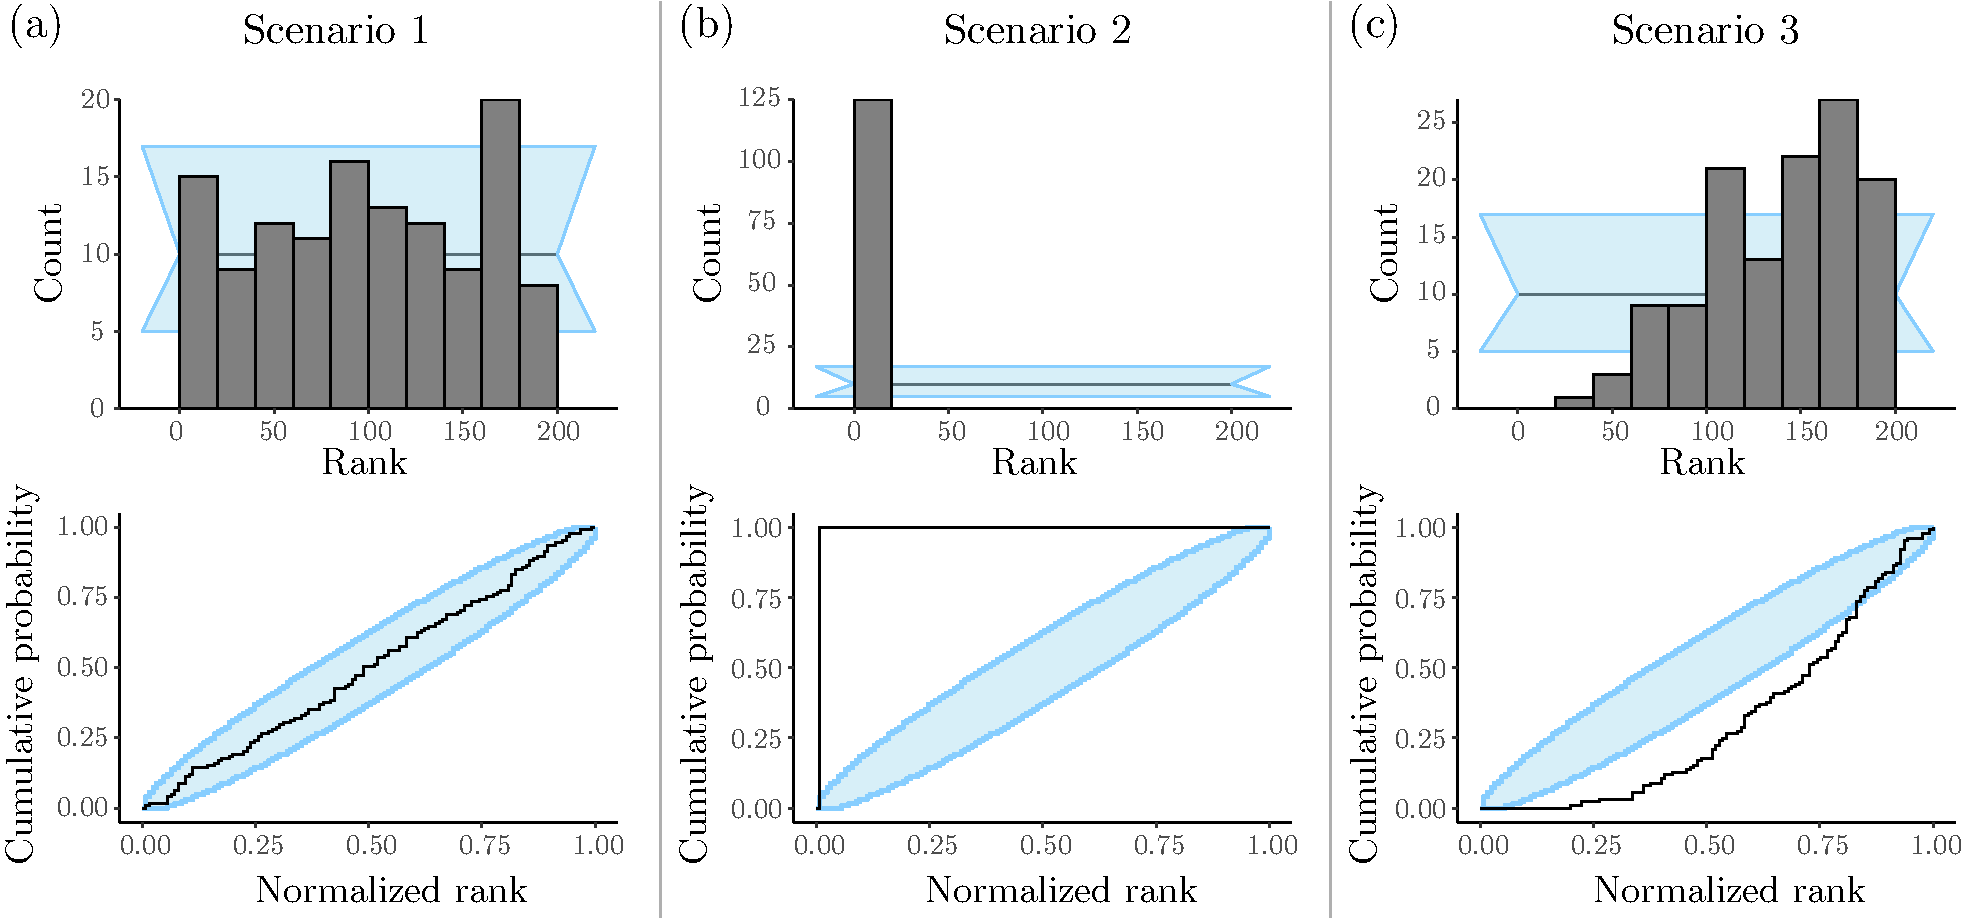
\includegraphics[width=\linewidth]{../figures/sbc_Yule_lambda_manual.pdf}
  \caption{Rank-uniformity validation (RUV) of the Bayesian hierarchical model in Fig. 1 in the main text.
    Panels in the top row show the histograms of $n=100$ ranks, for parameter $\Lambda$ in each scenario, obtained after 10\% burnin and thinning of posterior samples down to 200 out of 10,000.
    Panels in the bottom row show the corresponding ECDF plots, for parameter $\Lambda$ in each scenario.
    (a) In ``Scenario 1'', the model was correctly specified, and we simulated trees with 3 to 300 taxa using rejection sampling (approximately one in ten trees were rejected).
    (b) In ``Scenario 2'', the model was incorrectly specified in inference (see main text), and we used the same data sets simulated in ``Scenario 1''.
    (c) In ``Scenario 3'', the model was correctly specified, but rejection sampling was more intense (we rejected a large number of trees, approximately 90\%, keeping those having between 100 to 200 tips).
   }
  \label{supfig:ruv_yule_lambda}
\end{figure}

\begin{figure}[!ht]
  \centering
   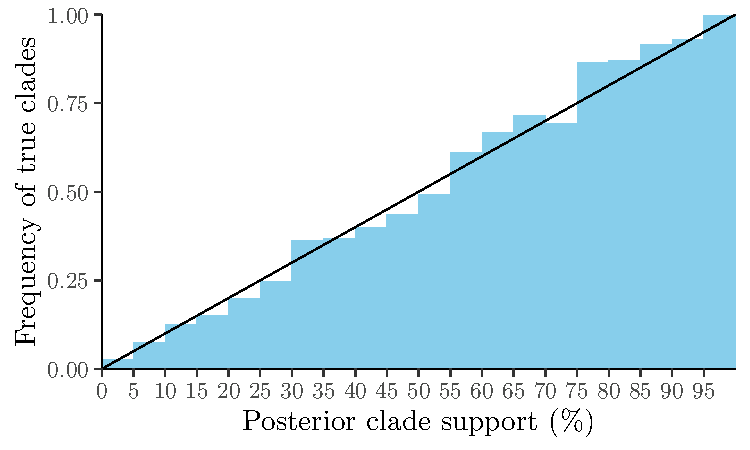
\includegraphics[width=8cm]{../figures/clade_coverage.pdf}
   \caption{Coverage validation in phylogenetic tree (topological) space. Bars represent the counts of true clades (in $n=100$ true, simulated trees) with their corresponding bin's posterior clade support, normalized by the total count of clades with that same posterior support value.}
   \label{supfig:clade_covg}
\end{figure}
 
\newpage

% \lstset{language=XML}
\section{Coverage validation using the Experimenter package for BEAST 2: a worked example}

\indent In this section we present a worked example of validation study using BEAST 2's Experimenter package.
We will start from working installations of BEAST 2 and the Experimenter package, which can be found on \url{https://github.com/christiaanjs/beast-validation/}.
Readers following along will also profit from having installed the \texttt{Tracer} \citep{tracer} and \texttt{LogCombiner} applications.

The hierarchical model whose implementation we will validate in this section is slightly more complex (and thus less pedagogical) than the one covered in the main manuscript, but more closely resembles a typical model employed by empirical phylogeneticists.
Much of the model specification will be familiar to this journal's readership.
For the sake of brevity, we leave the details on hyperprior specifications (parametric distributions) to the XML code snippets (those were commented so that they are human readable).

\subsection{Simulation}

\indent We will use BEAST 2's direct simulators to generate a set of phylogenetic trees under a Yule prior with normally distributed birth rates, $\lambda \sim \text{N}(1.0, 0.1)$.
Such a narrow normal prior constrains tree heights such that substitution rates are neither too low (i.e., we observe some phylogenetic signal) nor too high (i.e., we do not saturate our molecular alignments).
We shall assume a strict clock model with global substitution rate of 1.0.

Molecular alignments are simulated under an HKY model \citep{hky} with the transition to transversion rate, $\kappa$, being drawn from a log-normal distribution, and nucletotide frequencies, $\pi$, sampled from a Dirichlet prior.
Among-site substitution-rate variation is modeled with a discrete Gamma model \citep{yang94}, where the shape parameter is drawn from an exponential distribution.

\vspace{.25cm}

{\scriptsize
\begin{lstlisting}[language=XML, breaklines=true, backgroundcolor=\color{light-gray}]
<beast version="2.0" namespace="beast.pkgmgmt:beast.base.core:beast.base.inference:beast.base.evolution.alignment:beast.base.evolution.tree :beast.base.evolution.speciation:beast.base.inference.distribution:beast.base.inference.util :beast.base.inference.parameter">

    <run spec="DirectSimulator" nSamples="101">
        <distribution spec="CompoundDistribution" id="fullModel">
            <!-- Sampling the tree -->
            <distribution spec="YuleModel" id="yuleModel">
                <tree spec="Tree" id="Tree">
                    <taxonset spec="TaxonSet">
                        <plate var="n" range="t0,t1,t2,t3,t4,t5,t6,t7,t8,t9">
	                    <taxon spec="Taxon" id="$(n)"/>
	                </plate>
                    </taxonset>
                </tree>
                <birthDiffRate spec="RealParameter" id="birthRate" value="1.0"/>
            </distribution>

            <!-- Sampling the birth rate -->
            <distribution spec="beast.base.inference.distribution.Prior" id="birthDiffRatePrior">
                <x idref="birthRate"/>
                <distr spec="Normal" mean="4" sigma="0.1"/>
            </distribution>

            <!-- Sampling kappa for the HKY model -->
            <distribution spec="beast.base.inference.distribution.Prior" id="kappaPrior">
                <x spec="RealParameter" id="kappa" value="1.0"/>
                <distr spec="LogNormalDistributionModel" M="1.0" S="1.25"/>
            </distribution>

            <!-- Sampling the nucleotide frequencies for the HKY model -->
            <distribution id="FrequenciesPrior.s:dna" spec="beast.base.inference.distribution.Prior" >
               <x spec="RealParameter" id="freqParameter" value="0.25 0.25 0.25 0.25"/>
               <distr spec="Dirichlet" alpha="4.0 4.0 4.0 4.0"/>
            </distribution>

            <!-- Sampling the shape parameter of the discrete gamma model for rate heterogeneity -->
            <distribution spec="beast.base.inference.distribution.Prior" id="GammaShapePrior.s:dna">
                <x spec="RealParameter" id="gammaShape" lower="0.1" value="1.0"/>
            	<distr spec="Exponential" mean="1.0"/>
    	    </distribution>
        </distribution>

	<!-- Logging all sampled scalar values into file truth.log-->
        <logger logEvery="1" fileName="truth.log">
            <log id="TreeHeight" spec="beast.base.evolution.tree.TreeStatLogger" tree="@Tree"/>
            <log idref="birthRate"/>
            <log idref="kappa"/>
            <log idref="gammaShape"/>
            <log idref="freqParameter"/>
        </logger>

	<!-- Logging all sampled tree values into truth.trees-->
        <logger logEvery="1" fileName="truth.trees">
            <log idref="Tree"/>
        </logger>
    </run>
</beast>
\end{lstlisting}
}

As the XML file above specifies, we have BEAST 2 write all the sampled scalar and tree (``true'') values into log files \texttt{truth.xml} and \texttt{truth.trees}, respectively.
Inspecting the \texttt{truth.log} with the Tracer app reveals that the simulator works as expected (the means and variances of parameters match those specified in the XML file).
Note that we generated 101 samples ($n=100$ if we follow the main manuscript's notation; with an extra simulation for executing RUV in tree space), but nothing prevents users from generating more data sets.

At this point, the Experimenter package has the ``true'' simulated values it needs to populate an XML template 100 times.
The outcome will be 100 independent BEAST 2 runnable XML files for statistical inference.
The XML template looks like this:

\vspace{.25cm}

{\scriptsize
\begin{lstlisting}[language=XML, breaklines=true, backgroundcolor=\color{light-gray}]
<?xml version="1.0" encoding="UTF-8" standalone="no"?><beast beautitemplate='Standard' beautistatus='' namespace="beast.core:beast.evolution.alignment:beast.evolution.tree.coalescent:beast.core.util:beast.evolution.nuc:beast.evolution.operators:beast.evolution.sitemodel:beast.evolution.substitutionmodel:beast.base.evolution.alignment:beast.pkgmgmt:beast.base.core:beast.base.inference:beast.base.evolution.tree.coalescent:beast.pkgmgmt:beast.base.core:beast.base.inference.util:beast.evolution.nuc:beast.base.evolution.operator:beast.base.inference.operator:beast.base.evolution.sitemodel:beast.base.evolution.substitutionmodel:beast.base.evolution.likelihood" required="" version="2.7">

<!-- Alignment specifying the data type and taxa -->
<data id="input_alignment" spec="Alignment" name="alignment"  dataType="nucleotide">
    <plate var="n" range="t0,t1,t2,t3,t4,t5,t6,t7,t8,t9">
        <sequence id="seq_$(n)" taxon="$(n)" totalcount="4" value="?"/>
    </plate>
</data>

<!-- The simulated sequence alignment -->
<data spec='beastfx.app.seqgen.SimulatedAlignment' id="dna" sequencelength="$(sl=100)">
    <!-- The true tree down which sequences are simulated. -->
    <tree id="trueTree" spec='beast.base.evolution.tree.TreeParser' newick="$(tree)" IsLabelledNewick="true" adjustTipHeights="false" taxa="@input_alignment"/>

    <!-- Alignment block specified above -->
    <data idref="input_alignment"/>

    <!-- Site model used to simulate sequence data -->
    <siteModel id="trueSiteModel.s:dna" spec="SiteModel" gammaCategoryCount="4" proportionInvariant="0.0" mutationRate="1.0">

        <!-- Discrete Gamma shape parameter value will be replaced by the true value -->
        <parameter id="truegammaShape.s:dna" spec="parameter.RealParameter"  name="shape">$(gammaShape)</parameter>
        
        <!-- Kappa and nucleotide frequency values will be replaced by the true values -->
        <substModel id="trueHKY.s:big2_barcs" spec="HKY" kappa="$(kappa)">
            <frequencies id="trueFreqs.s:dna" spec="Frequencies" frequencies="$(freqParameter.1) $(freqParameter.2)  $(freqParameter.3) $(freqParameter.4)"/>
        </substModel>
    </siteModel> 
      
    <!-- We use a strict clock with rate fixed to 1.0 -->
    <branchRateModel id="trueStrictClock.c:cytb" spec="beast.base.evolution.branchratemodel.StrictClockModel" clock.rate="1.0"/>
 </data>
 
 <!--
 	The rest of the XML comes from a BEAUti generated XML that is too long to
 	include here. The full file can be found here:
	https://github.com/rbouckaert/DeveloperManual/blob/master/examples/yule/input.xml
 -->
\end{lstlisting}
}

Here, we can use the \texttt{CoverageTestXMLGenerator2} utility that comes with the Experimenter package to generate the 100 BEAST XML files.
It can be run from the shell or Terminal application as follows:

\vspace{.25cm}

{\scriptsize
\begin{lstlisting}[language=bash]
applauncher CoverageTestXMLGenerator2 -workingDir . -out xml -log truth.log -tree truth.trees -xml input.xml 
\end{lstlisting}
}

\noindent (Note that application \texttt{applauncher} above is part of BEAST 2, and that it must be in the \texttt{PATH} environmental variable of the Terminal to be run as specified.)
This command generates a directory called \texttt{xml/} with files called \texttt{analysis-out0.xml} to \texttt{analysis99.xml}.
It can be useful to make a subdirectory \texttt{run1/} inside the \texttt{xml} directory for the occasion of failed or alternative experiments (e.g., longer MCMC chains).

\subsection{Statistical inference}

Inside the \texttt{run1/} directory, we can run the 100 XML files from the Terminal:

\vspace{.25cm}

{\scriptsize
\begin{lstlisting}[language=bash]
for i in  {0..99}; do beast -seed 127$i -overwrite ../analysis-out$i.xml > out$i 2>&1 ; done 
\end{lstlisting}
}

Once the BEAST 2 runs have finished, we then use the \texttt{LogCombiner} application to summarize the parameter estimates in a single file:

\vspace{.25cm}

{\scriptsize
\begin{lstlisting}[language=bash]
loganalyser -oneline *log > summary
\end{lstlisting}
}

\subsection{Calculating and visualizing coverage}

After statistical inference, we can run the \texttt{CoverageCalculator} tool (part of the Experimenter package) from the Terminal to produce coverage summary statistics:

\vspace{.25cm}

{\scriptsize
\begin{lstlisting}[language=bash, breaklines=true]
applauncher beastvalidation.experimenter.CoverageCalculator -log ../../truth.log -logA summary -out /tmp -showRho true -showESS false -showMean false 
\end{lstlisting}
}

% \caption
The Terminal output of coverage calculator in the Experimenter package for BEAST 2 is shown in supplementary figure \ref{supfig:terminal}.
An asterisk is added next to the coverage column if it has a value outside the expected range.
Here $\kappa$ is marked, and judging from the low effective sample size (see \texttt{Min ESS} column) this can be fixed by running the MCMC chains longer.
The Experimenter package should further output graphs for scalar parameters as shown in supplementary figure \ref{supfig:experimenter}.

\begin{figure}
  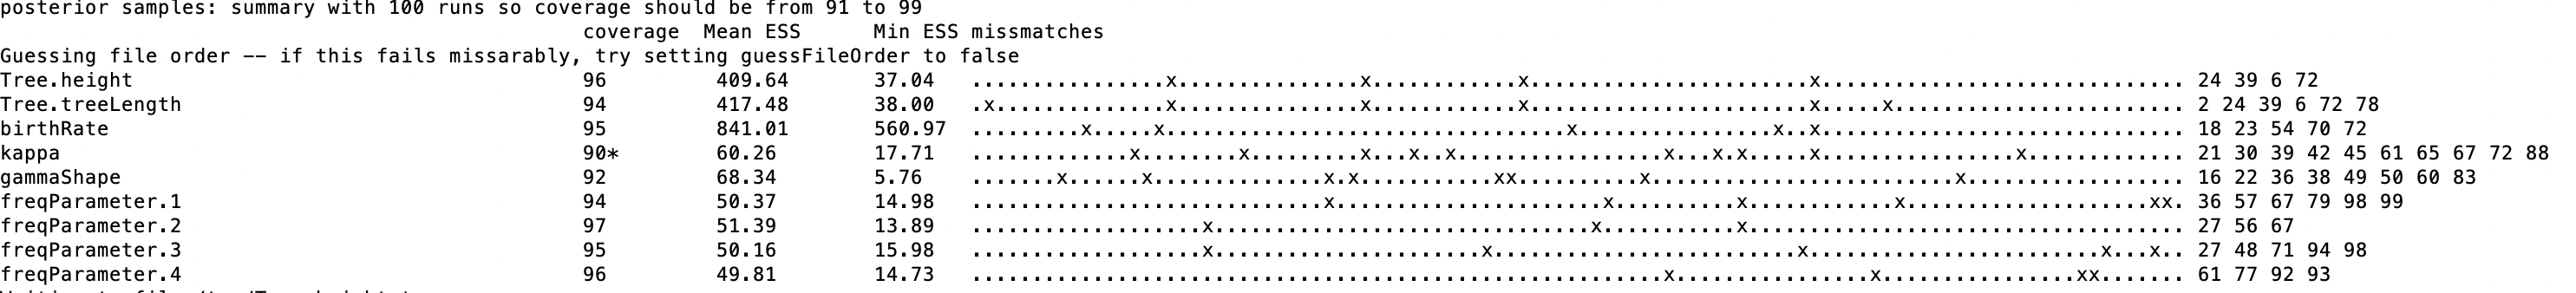
\includegraphics[width=\textwidth]{../figures/coveragecalculator0.png}
  \caption{Terminal output of the \texttt{CoverageCalculator} application/}
  \label{supfig:terminal}
\end{figure}

\begin{figure}
   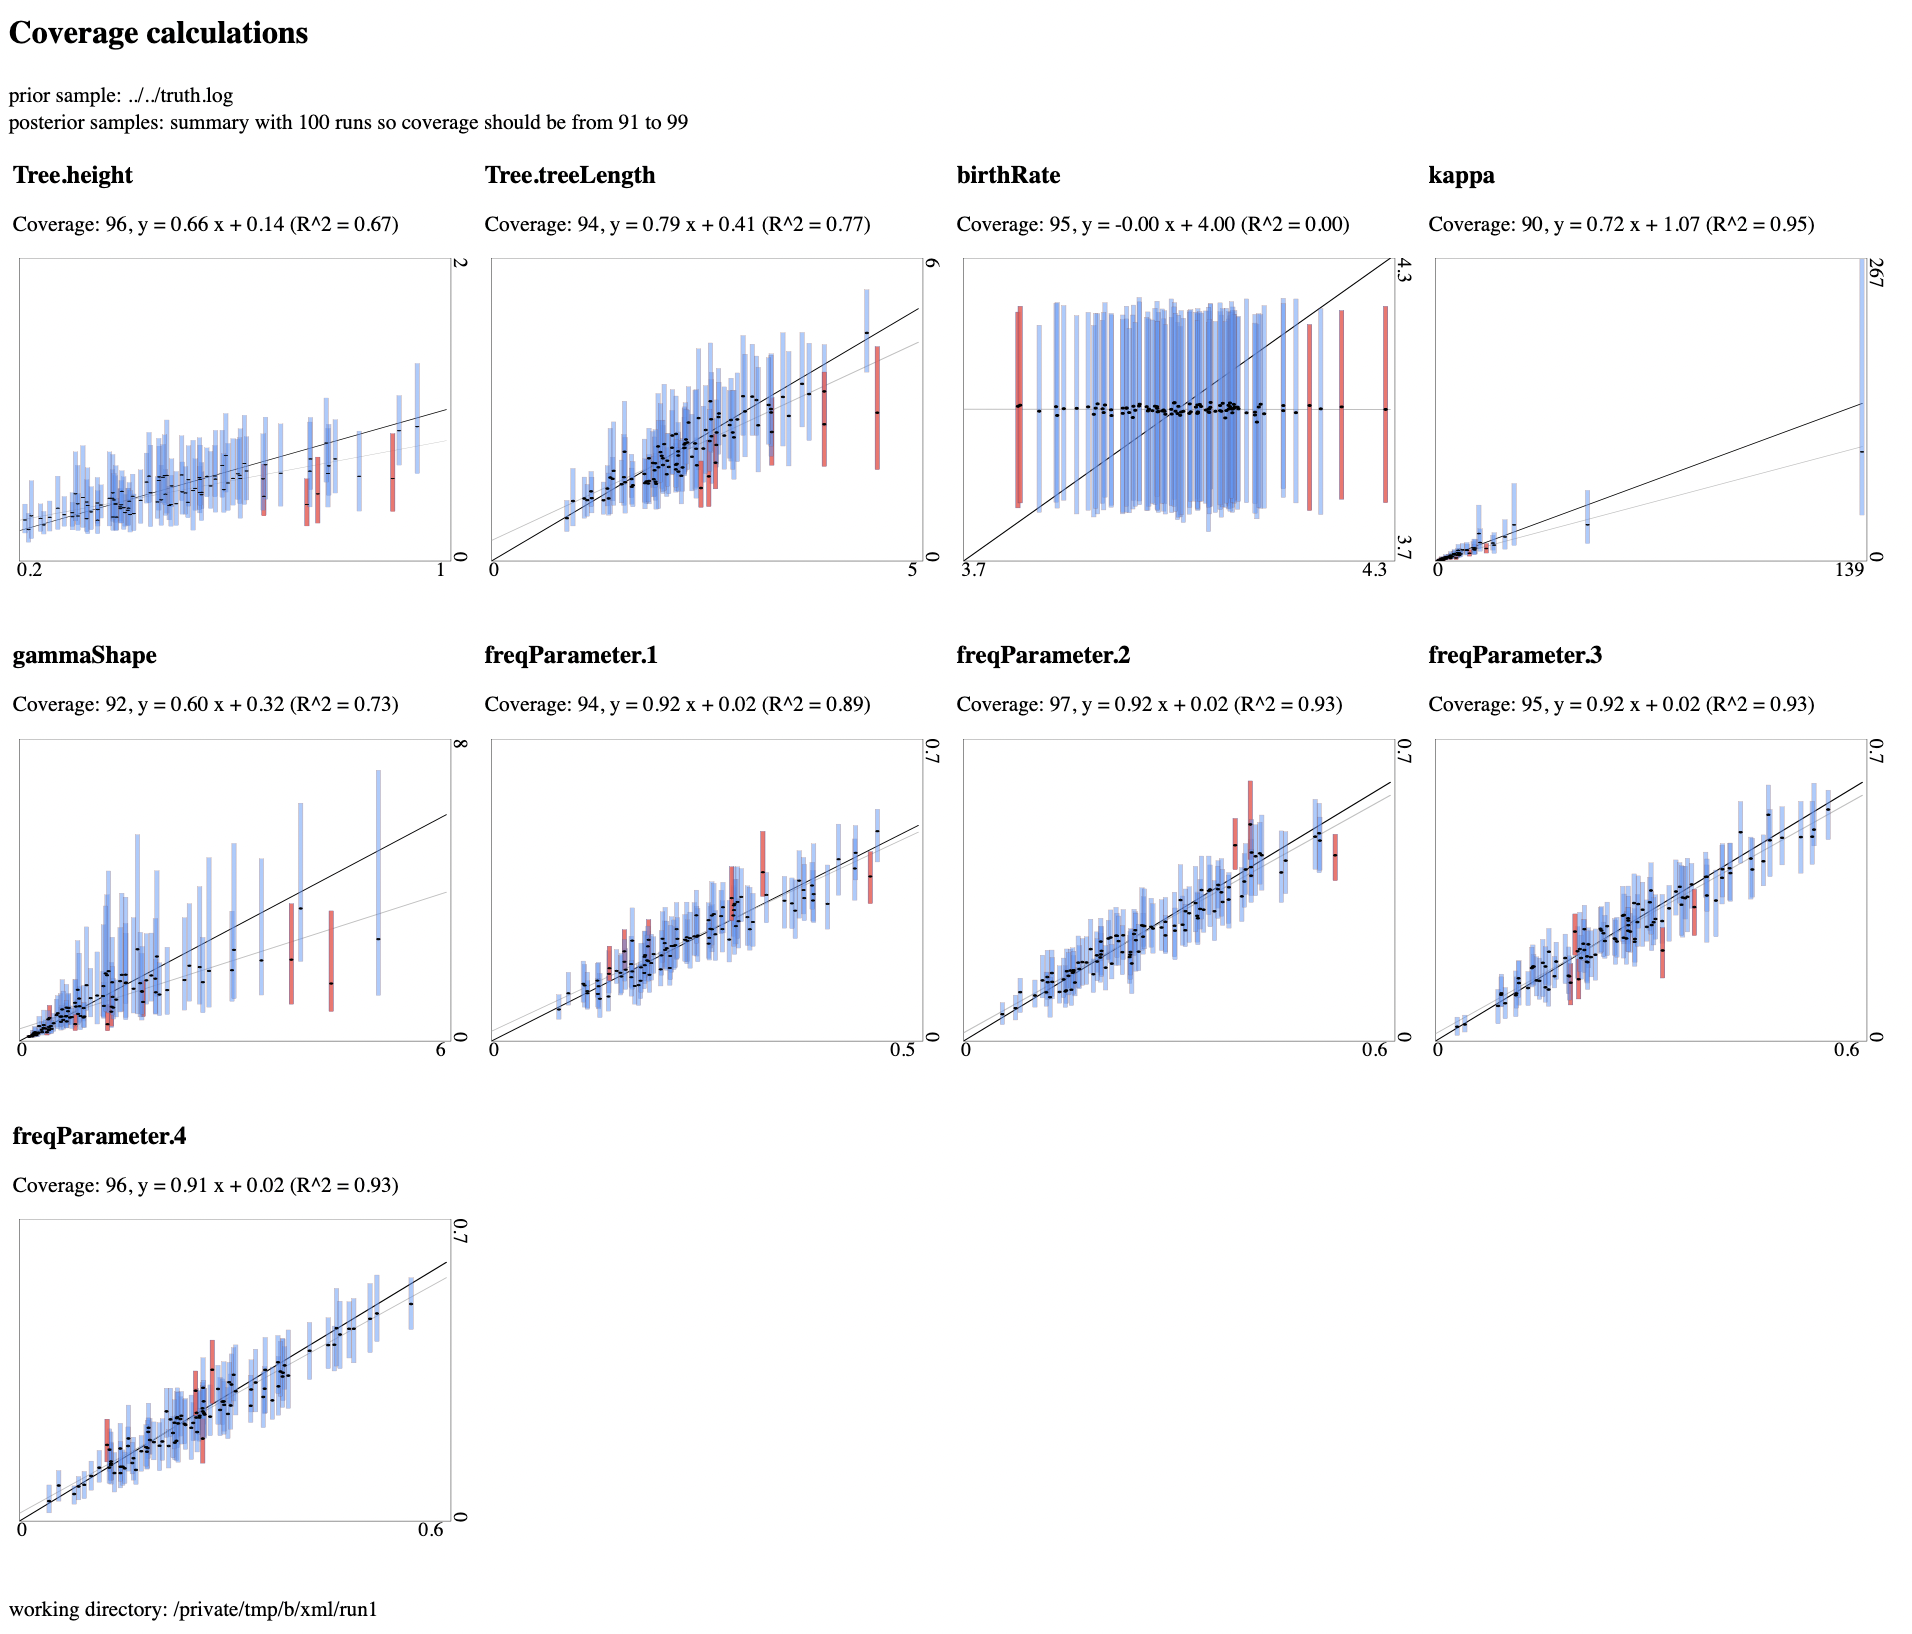
\includegraphics[width=\textwidth]{../figures/coveragecalculator.png}
   \caption{
     Graphs show the $x=y$ line in black and linear regression lines through the medians in gray.
     The regression lines and $R^2$ values indicate the influence of the prior vs. that of the likelihood over the parameter estimates.
     A low $R^2$ (e.g., birth rate) suggests the prior has more influence while a high $R^2$ (e.g., nucleotide frequencies) suggests the data has more influence on estimates.
   }
   \label{supfig:experimenter}
\end{figure}

Finally, we look at clade coverages, which can be calculated using the \texttt{CladeCoverageCalculator} application in the Experimenter package:

\vspace{.25cm}

{\scriptsize
\begin{lstlisting}[language=bash]
applauncher CladeCoverageCalculator -tru ../../truth.trees -pref analysis-out -png coverage.png -bins 10
\end{lstlisting}
}

This command executes the procedure described at the end of section 6, producing the graph illustrated by supplementary figure \ref{supfig:clade_covg}.

\begin{figure}
  \centering
  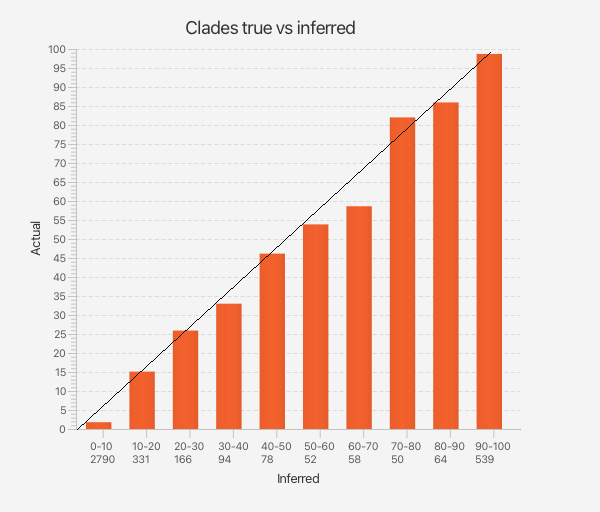
\includegraphics[width=0.5\textwidth]{../figures/experimentercoverage.png}
  \caption{Clade coverages for the worked example using BEAST 2's Experimenter package.}
\end{figure}

\subsection{RUV validation}

To do an RUV analysis, we must first combine the log files produced during inference into a single file:

\vspace{.25cm}

{\scriptsize
\begin{lstlisting}[language=bash]
logcombiner -b 10 -log analysis-out?.log analysis-out??.log -o combined.log
\end{lstlisting}
}

Next, we create summary statistics using the \texttt{SBCAnalyser} tool that is part of the Experimenter package:

\vspace{.25cm}

{\scriptsize
\begin{lstlisting}[language=bash]
applauncher SBCAnalyser -log ../../truth.log -logA combined.log -out /tmp -bins 10
\end{lstlisting}
}

The Terminal output is shown in supplementary figure \ref{supfig:terminal2}; it displays the bin counts as well as ECDF plots (not all of them shown due to size of screen display).
We can also graphically summarize the RUV procedure (Supplementary Fig. \ref{supfig:experimenterruv}).

\begin{figure}
  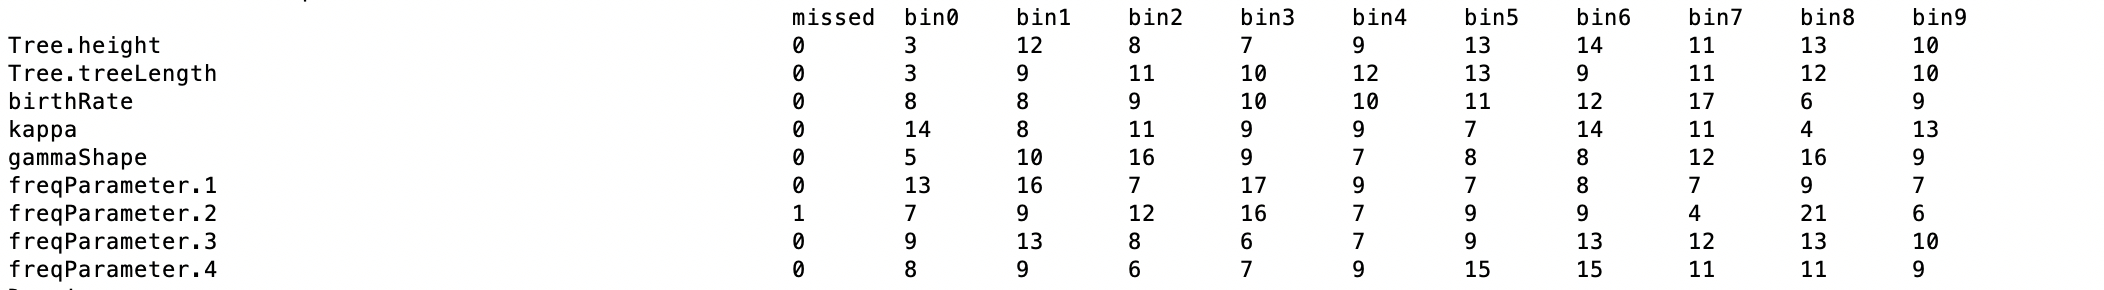
\includegraphics[width=\textwidth]{../figures/sbscalculator0.png}
  \caption{Frequency parameter 2 has one bin that is outside the expected range (indicated by the missed bin column).}
  \label{supfig:terminal2}
\end{figure}

\begin{figure}
  \centering
  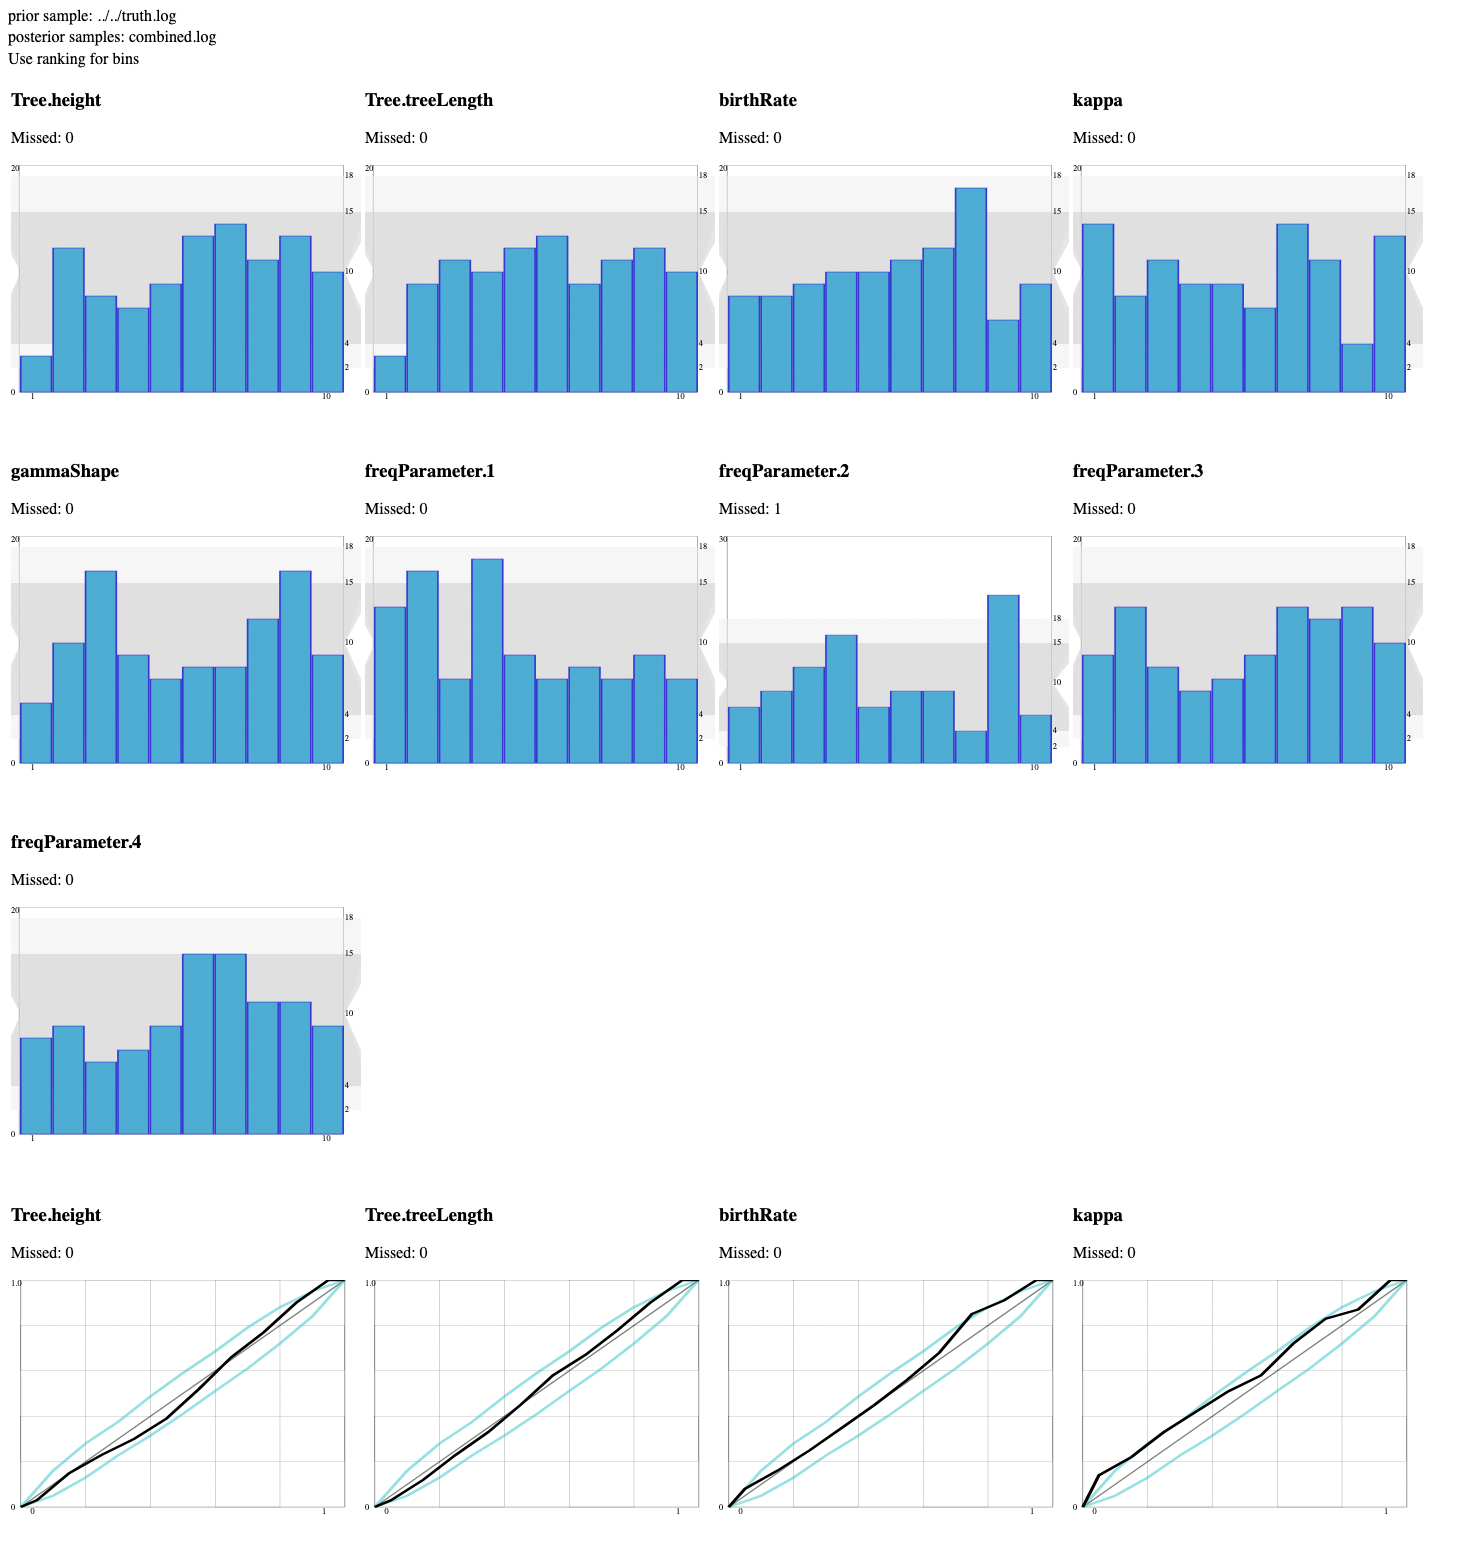
\includegraphics[width=\textwidth]{../figures/sbscalculator.png}
  \caption{Rank histograms and ECDF plots for the worked example using BEAST 2's Experimenter package.}
  \label{supfig:experimenterruv}
\end{figure}

More details on the tools used above can be found on \url{https://github.com/rbouckaert/DeveloperManual/}.

\clearpage

\bibliography{refs}

\end{document}
